\addtocontents{toc}{\protect\newpage}
\chapter{Design Phase} \label{chap:design}

{This chapter sums up typical use cases for instructors, solvers and both (general). Each use case contains preconditions, the actual flow and possibly an alternative flow. Consecutively it includes all use cases in process activity diagrams. The last section shows what use cases are covered by which processes (and vice versa).}

\section{Use Cases} \label{sec:uc}

\subsection{{Instructor Use Cases {[}IUC{]}}} \label{ssec:iuc}

\subsubsection{{[}IUC1{]} Create new GitLab working project}

\begin{itemize}
\item
  {Preconditions}
    \begin{enumerate}
    \item 
      {Working project with proper documentation and tests.}
    \item
      {Granted access to instructor's group in root namespace (group), \\ e.g. \texttt{umiami/george}.}
    \end{enumerate}
\end{itemize}

\begin{itemize}
\item
  {Flow}
    \begin{enumerate}
    \item
      {Instructor creates a new (course) namespace, e.g. \texttt{umiami/george/csc220}.}
    \item
      {Instructor creates a new empty GitLab project repository in the created namespace, e.g. \texttt{umiami/george/csc220/lab01}.}
    \item
      {Instructor sets CI variable \texttt{ACCESS\_TOKEN} into the created project.}
    \item
      {Instructor integrates CA evaluation into the project's CI}
    \item
      {Instructor adds links to badges into the \texttt{README} file.}
    \item
      {Instructor pushes the working project into the newly created repository.}
    \end{enumerate}
\end{itemize}

\subsubsection{{[}IUC4{]} Create an assignment from the working project}

\begin{itemize}
\item
  {Preconditions}
    \begin{enumerate}
    \item
      {IUC1}
    \end{enumerate}
\end{itemize}

\begin{itemize}
\item
  {Flow}
    \begin{enumerate}
    \item
      {Instructor creates a protected branch for project assignment and switches to it, e.g. \texttt{fall20}.}
    \item
      {Instructor adds instructions into the \texttt{README} file or in a form of issues with an \texttt{assignment} label.}
    \item
      {Instructor removes chunks of codes in reverse to the instructions.}
    \item
      {Instructor updates badge links in the \texttt{README} file to the current branch.}
    \item
      {Instructor pushes the assignment project into the newly created branch.}
    \end{enumerate}
\end{itemize}

\subsubsection{{[}IUC5{]} Distribute the assignment among solvers}

\begin{itemize}
\item
  {Preconditions}
    \begin{enumerate}
    \item
      {Protected \texttt{ACCESS\_TOKEN} variable accessible from project.}
    \item
      {IUC4}
    \end{enumerate}
\end{itemize}

\begin{itemize}
\item
  {Flow}
    \begin{enumerate}
    \item
      {Instructor integrates CA distribution CI into the assignment branch.}
    \item
      {Instructor manually executes the CI distribution pipeline to create solver assignments.}
    \item
      {CA script distributes (creates or updates) solver repositories.}
    \end{enumerate}
\end{itemize}

\subsubsection{{[}IUC6{]} Update solver assignments}

\begin{itemize}
\item
  {Preconditions}
    \begin{enumerate}
    \item
      {IUC5}
    \item
      {Updated content on the assignment branch including adding solver usernames.}
    \end{enumerate}
\end{itemize}

\begin{itemize}
\item
  {Flow}
    \begin{enumerate}
    \item
      {Instructor manually runs the CI distribution pipeline to update existing and create new solver assignments.}
    \end{enumerate}
\end{itemize}

\subsubsection{{[}IUC7{]} Collective similarity measure}

\begin{itemize}
\item
  {Preconditions}
    \begin{enumerate}
    \item
      {IUC5}
    \end{enumerate}
\end{itemize}

\begin{itemize}
\item
  {Flow}
    \begin{enumerate}
    \item
      {Instructor integrates CA measure CI into the main project branch.}
    \item
      {Instructor manually executes CI measure pipeline.}
    \item
      {Instructor navigates into the generated Moss URL with results.}
    \end{enumerate}
\end{itemize}

\subsubsection{{[}IUC8{]} Collective evaluation status}

\begin{itemize}
\item
  {Preconditions}
    \begin{enumerate}
    \item
      {IUC5}
    \end{enumerate}
\end{itemize}

\begin{itemize}
\item
  {Flow}
    \begin{enumerate}
    \item
      {Instructor integrates CA collective CI into the project's main branch.}
    \item
      {Instructor manually executes CI collective CI pipeline.}
    \item
      {GitLab CI displays results in pipeline output.}
    \item
      {Instructor manually downloads complete results from GitLab CI.}
    \end{enumerate}
\end{itemize}

\subsubsection{{[}IUC10{]} Collective download}

\begin{itemize}
\item
  {Precondition}
    \begin{enumerate}
    \item
      {IUC8}
    \end{enumerate}
\end{itemize}

\begin{itemize}
\item
  {Flow}
    \begin{enumerate}
    \item
      {Instructor downloads artifacts from GitLab.}
    \end{enumerate}
\end{itemize}

\subsubsection{{[}IUC11{]} View solution diff with working project}

\begin{itemize}
\item
  {Precondition}
    \begin{enumerate}
    \item
      {IUC5}
    \item
      {Working project stored locally, e.g. in \texttt{\textapprox/lab01-project}}
    \end{enumerate}
\end{itemize}

\begin{itemize}
\item
  {Flow}
    \begin{enumerate}
    \item
      {Instructor downloads Solver's assignment repository, \\ e.g. into \texttt{\textapprox/lab01-vjm001}}
    \item
      {Instructor shows changes between original project and Solver's assignment by running \texttt{git diff -\/-no-index \textapprox/lab01-project \textapprox/lab01-vjm001}.}
    \end{enumerate}
\end{itemize}

\subsection{General Use Cases {[}GUC{]}} \label{ssec:guc}

\subsubsection{{[}GUC1{]} Check evaluation status}

\begin{itemize}
\item
  {Preconditions}
    \begin{enumerate}
    \item
      {GUC3}
    \end{enumerate}
\end{itemize}

\begin{itemize}
\item
  {Flow}
    \begin{enumerate}
    \item
      {User navigates into the GitLab assignment project and reads project bad\-ges.}
    \item
      {User can click on a specific badge to see a log file with complete information.}
    \end{enumerate}
\end{itemize}

\subsubsection{{[}GUC3{]} Generate status badges}

\begin{itemize}
\item
  {Preconditions}
    \begin{enumerate}
    \item
      {IUC1 or IUC4 or IUC5 or SUC2 or SUC3}
    \end{enumerate}
\end{itemize}

\begin{itemize}
\item
  {Flow}
    \begin{enumerate}
    \item
      {GitLab CI runs CA evaluation.}
    \item
      {CA evaluation script generates badges.}
    \end{enumerate}
\end{itemize}

\subsubsection{{[}GUC4{]} Providing remote support}

\begin{itemize}
\item
  {Preconditions}
    \begin{enumerate}
    \item
      {IUC5}
    \end{enumerate}
\end{itemize}

\begin{itemize}
\item
  {Flow}
    \begin{enumerate}
    \item
      {Solver navigates into the GitLab assignment Issues.}
    \item
      {Solver creates a new issue describing the problem mentioning an instructor in description by adding \texttt{@instructor\_username}.}
    \item
      {GitLab notifies the instructor.}
    \item
      {Instructor provides remote support by adding a reply.}
    \item
      {GitLab notifies the solver.}
    \end{enumerate}
\end{itemize}

\subsubsection{{[}GUC5{]} View solution diff with original assignment locally}

\begin{itemize}
\item
  {Preconditions}
    \begin{enumerate}
    \item
      {IUC5}
    \end{enumerate}
\end{itemize}

\begin{itemize}
\item
  {Flow}
    \begin{enumerate}
    \item
      {User clones GitLab assignment project.}
    \item
      {User shows changes between solution and original assignment by running \texttt{git diff source}.}
    \end{enumerate}
\end{itemize}

\subsubsection{{[}GUC6{]} View solution diff with original assignment online}

\begin{itemize}
\item
  {Preconditions}
    \begin{enumerate}
    \item
      {IUC5}
    \end{enumerate}
\end{itemize}

\begin{itemize}
\item
  {Flow}
    \begin{enumerate}
    \item
      {User navigates into the GitLab assignment project.}
    \item
      {User navigates into the Compare page.}
    \item
      {User selects the \texttt{source} branch as a target.}
    \end{enumerate}
\end{itemize}

\subsection{Solver Use Cases {[}SUC{]}} \label{ssec:suc}

\subsubsection{{[}SUC1{]} Process assignment update}

\begin{itemize}
\item
  {Preconditions}
    \begin{enumerate}
    \item
      {IUC6}
    \end{enumerate}
\end{itemize}

\begin{itemize}
\item
  {Flow}
    \begin{enumerate}
    \item
      {Solver navigates into the GitLab assignment merge requests.}
    \item
      {Solver opens a merge request labeled by \texttt{Update from source branch}.}
    \item
      {Solver views merge request modifications by clicking on the \texttt{Changes} tab.}
    \item
      {Solver accepts the merge request by pressing the \texttt{Merge} button on the \texttt{Overview} page.}
    \end{enumerate}
\item
  {Alternative flow d1}
    \begin{enumerate}
    \item
      {Solver comments the merge request with mentioning Instructor \\ by \texttt{@instructor\_username}.}
    \end{enumerate}
\end{itemize}

\subsubsection{{[}SUC2{]} Edit assignment online}

\begin{itemize}
\item
  {Preconditions}
    \begin{enumerate}
    \item
      {IUC5}
    \end{enumerate}
\end{itemize}

\begin{itemize}
\item
  {Flow}
    \begin{enumerate}
    \item
      {Solver edits a file using GitLab browser UI.}
    \item
      {Solver double-checks modifications.}
    \item
      {Solver commits changes with a commit message.}
    \item
      {GitLab pushes the commit into the GitLab repository.}
    \item
      {GitLab runs ca evaluation and updates status badges.}
    \end{enumerate}
\end{itemize}

\subsubsection{{[}SUC3{]} Edit assignment locally}

\begin{itemize}
\item
  {Preconditions}
    \begin{enumerate}
    \item
      {IUC5}
    \end{enumerate}
\end{itemize}

\begin{itemize}
\item
  {Flow}
    \begin{enumerate}
    \item
      {Solver clones or updates (pulls) the project into the local repository.}
    \item
      {Solver edits a file using favorite editor and saves changes.}
    \item
      {Solver double-checks modifications using editor or CLI.}
    \item
      {Solver checks if the script compiles and runs.}
    \item
      {Solver checks if tests are passing.}
    \item
      {Solver commits changes with a commit message.}
    \item
      {Solver pushes the project into the GitLab repository.}
    \item
      {GitLab runs ca evaluation and updates status badges.}
    \end{enumerate}
\end{itemize}

\section{Process Activity Diagrams} \label{sec:ad}

\subsection{{[}AD1{]} Distribute assignment} \label{ssec: ad1}

\begin{figure}[H]
    \centering
    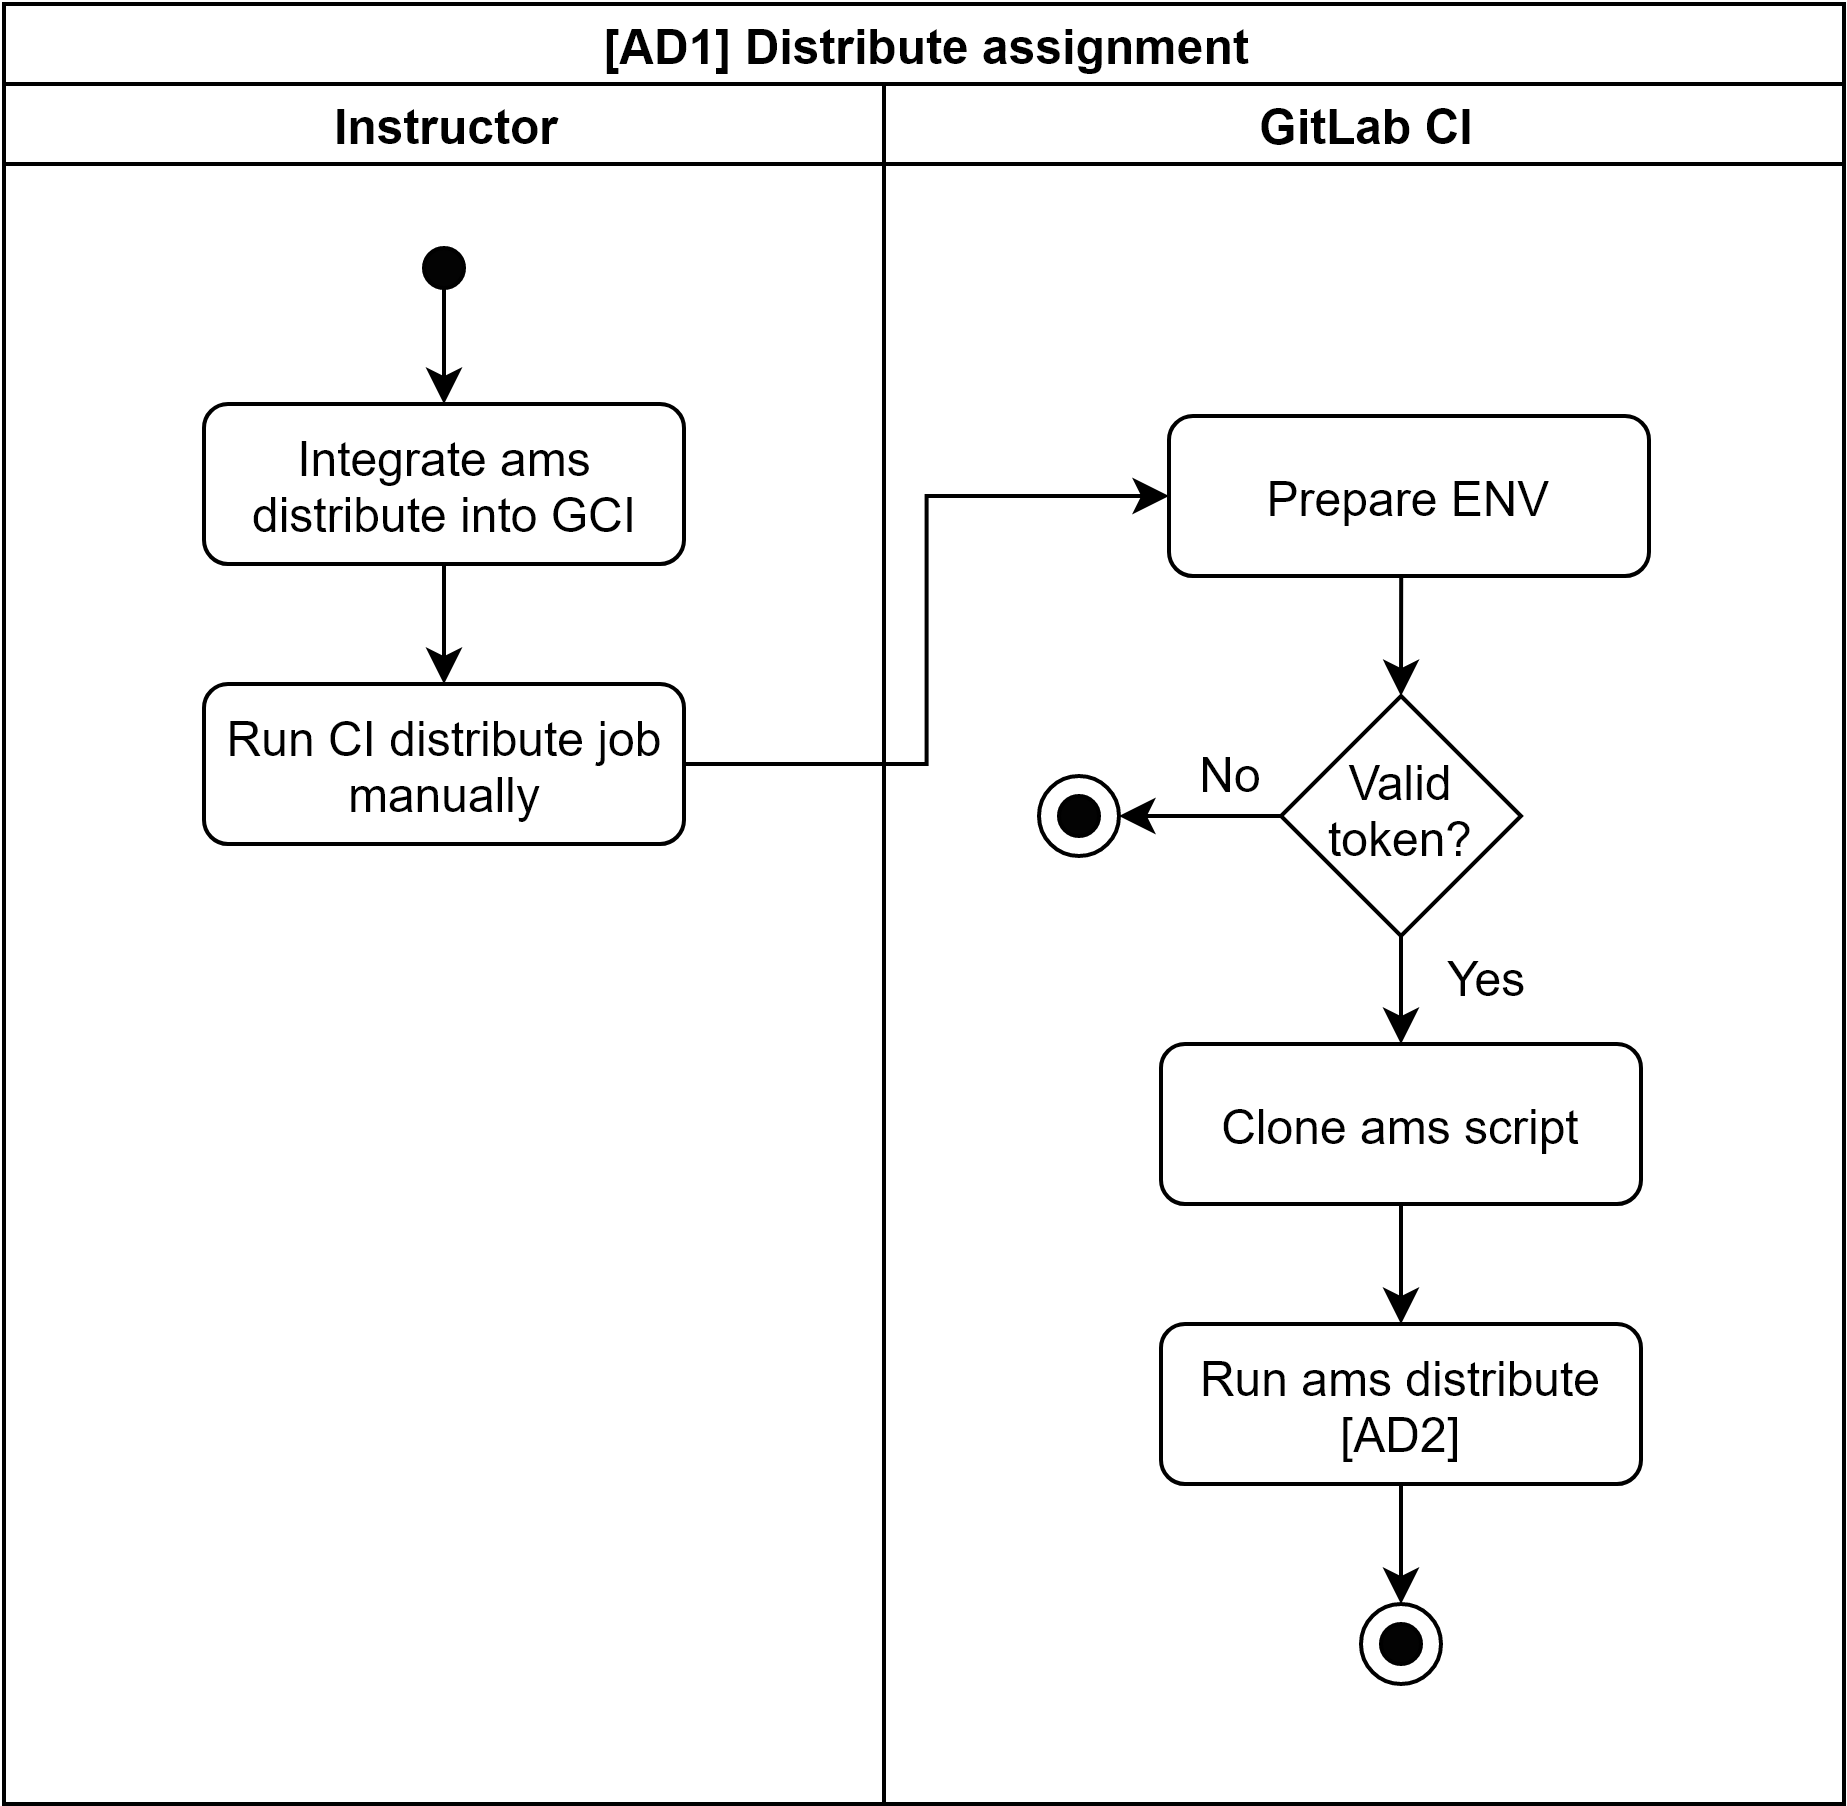
\includegraphics[width=\textwidth,height=\textheight,keepaspectratio]{Figures/ad/ad4.png}
    \caption{Distribute assignment activity diagram}
\end{figure}

\subsection{{[}AD2{]} AMS distribute} \label{ssec:ad2}

\begin{figure}[H]
    \centering
    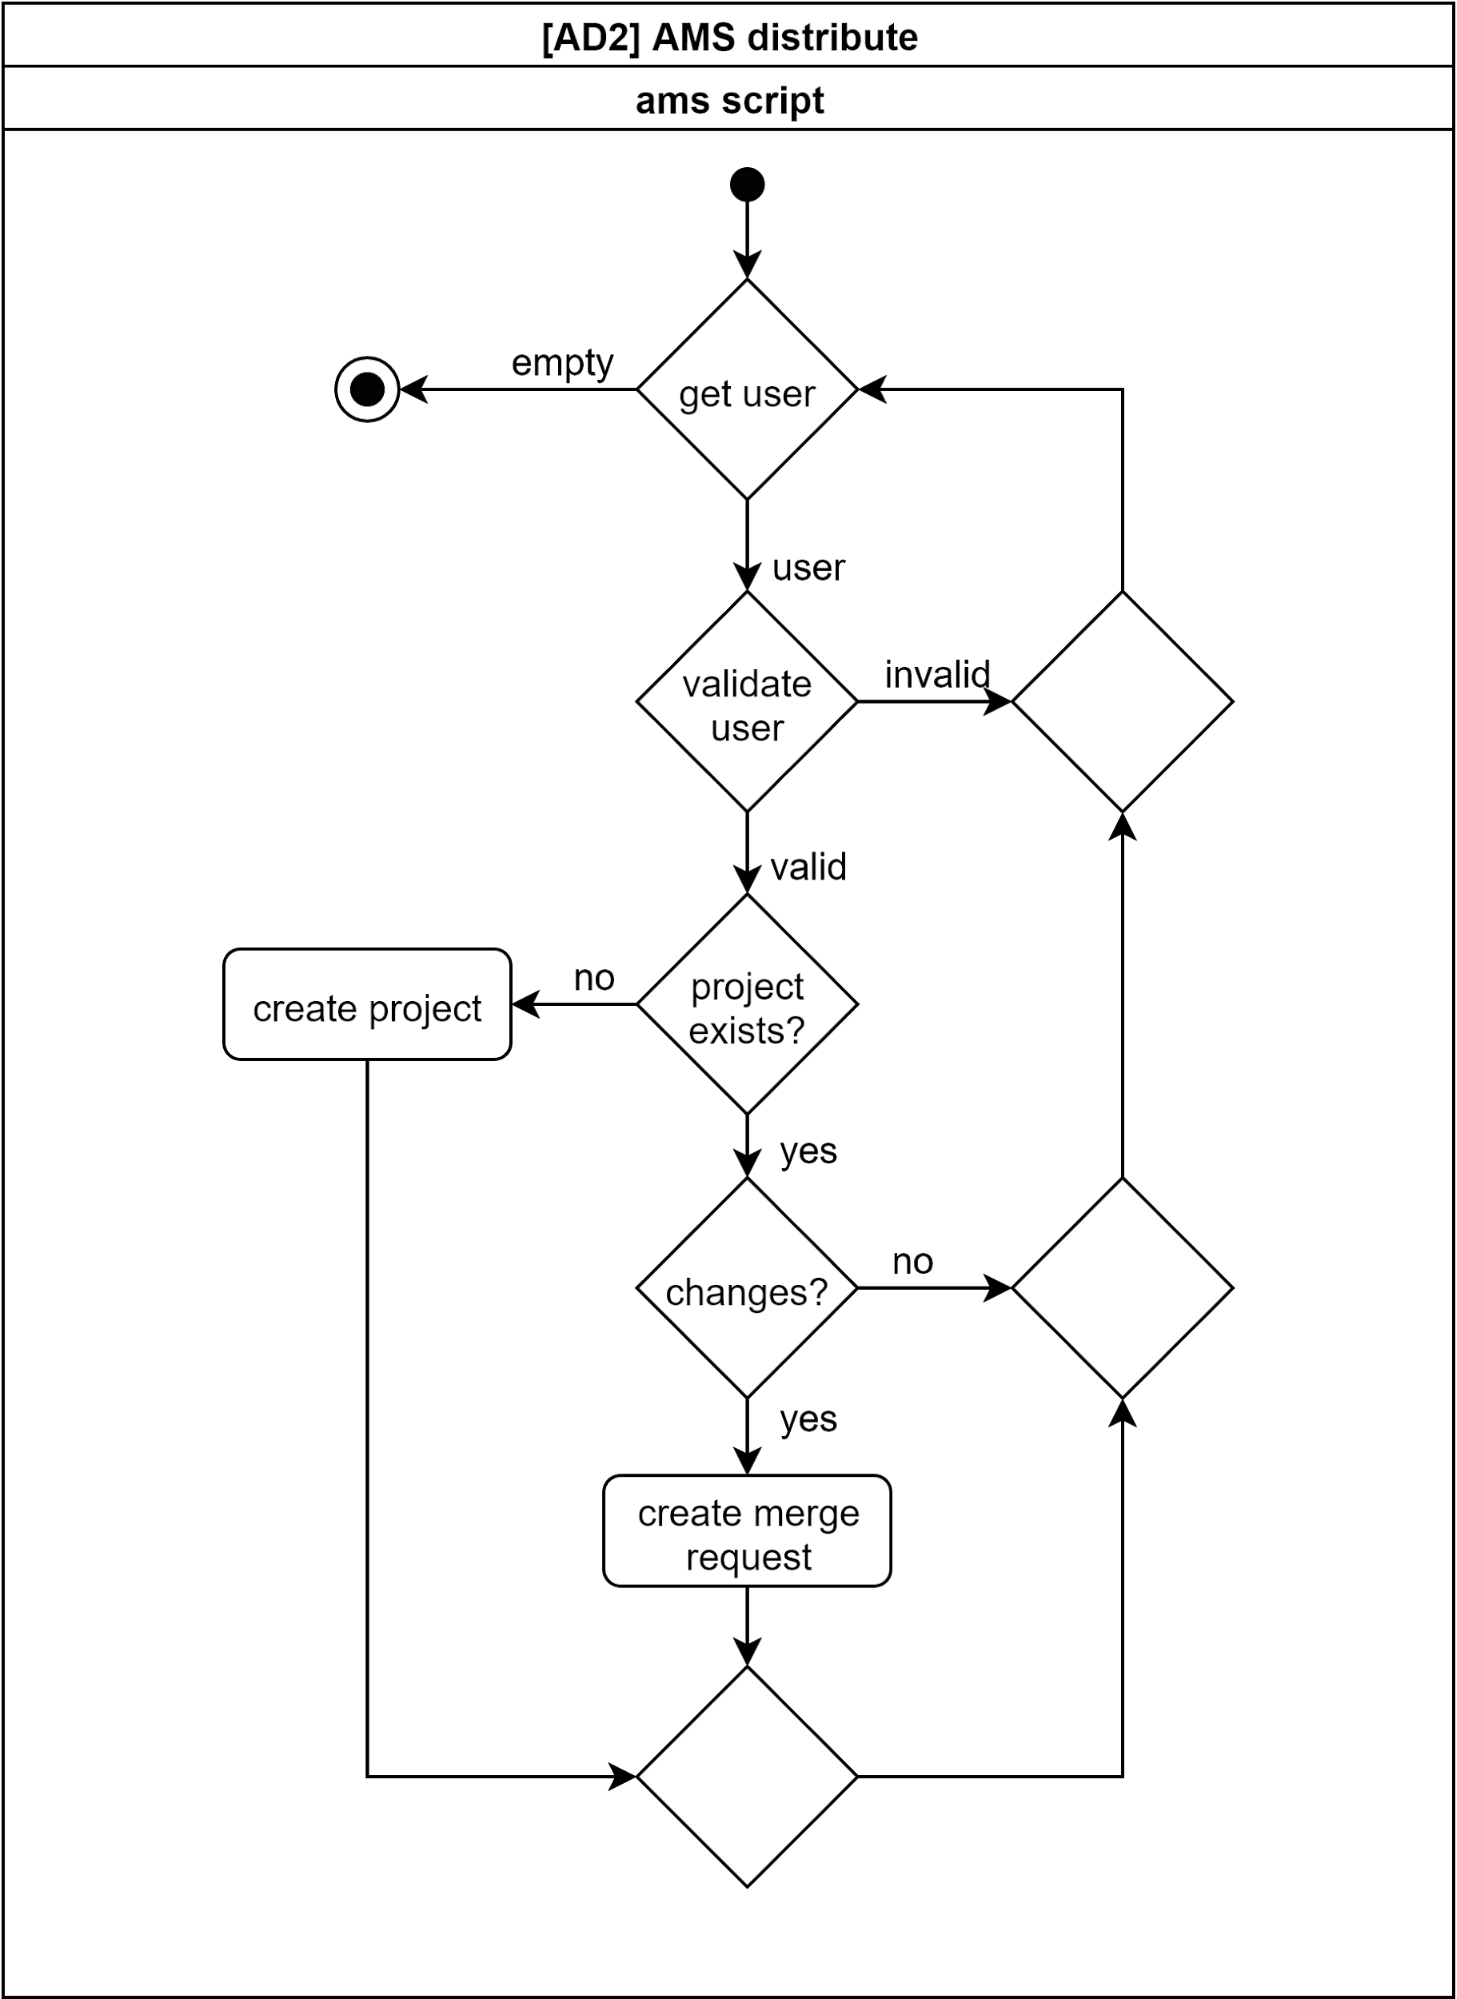
\includegraphics[width=\textwidth,height=.8\textheight,keepaspectratio]{Figures/ad/ad1.png}
    \caption{AMS distribute activity diagram}
\end{figure}

\subsection{{[}AD3{]} Evaluate Assignment} \label{ssec:ad3}

\begin{figure}[H]
    \centering
    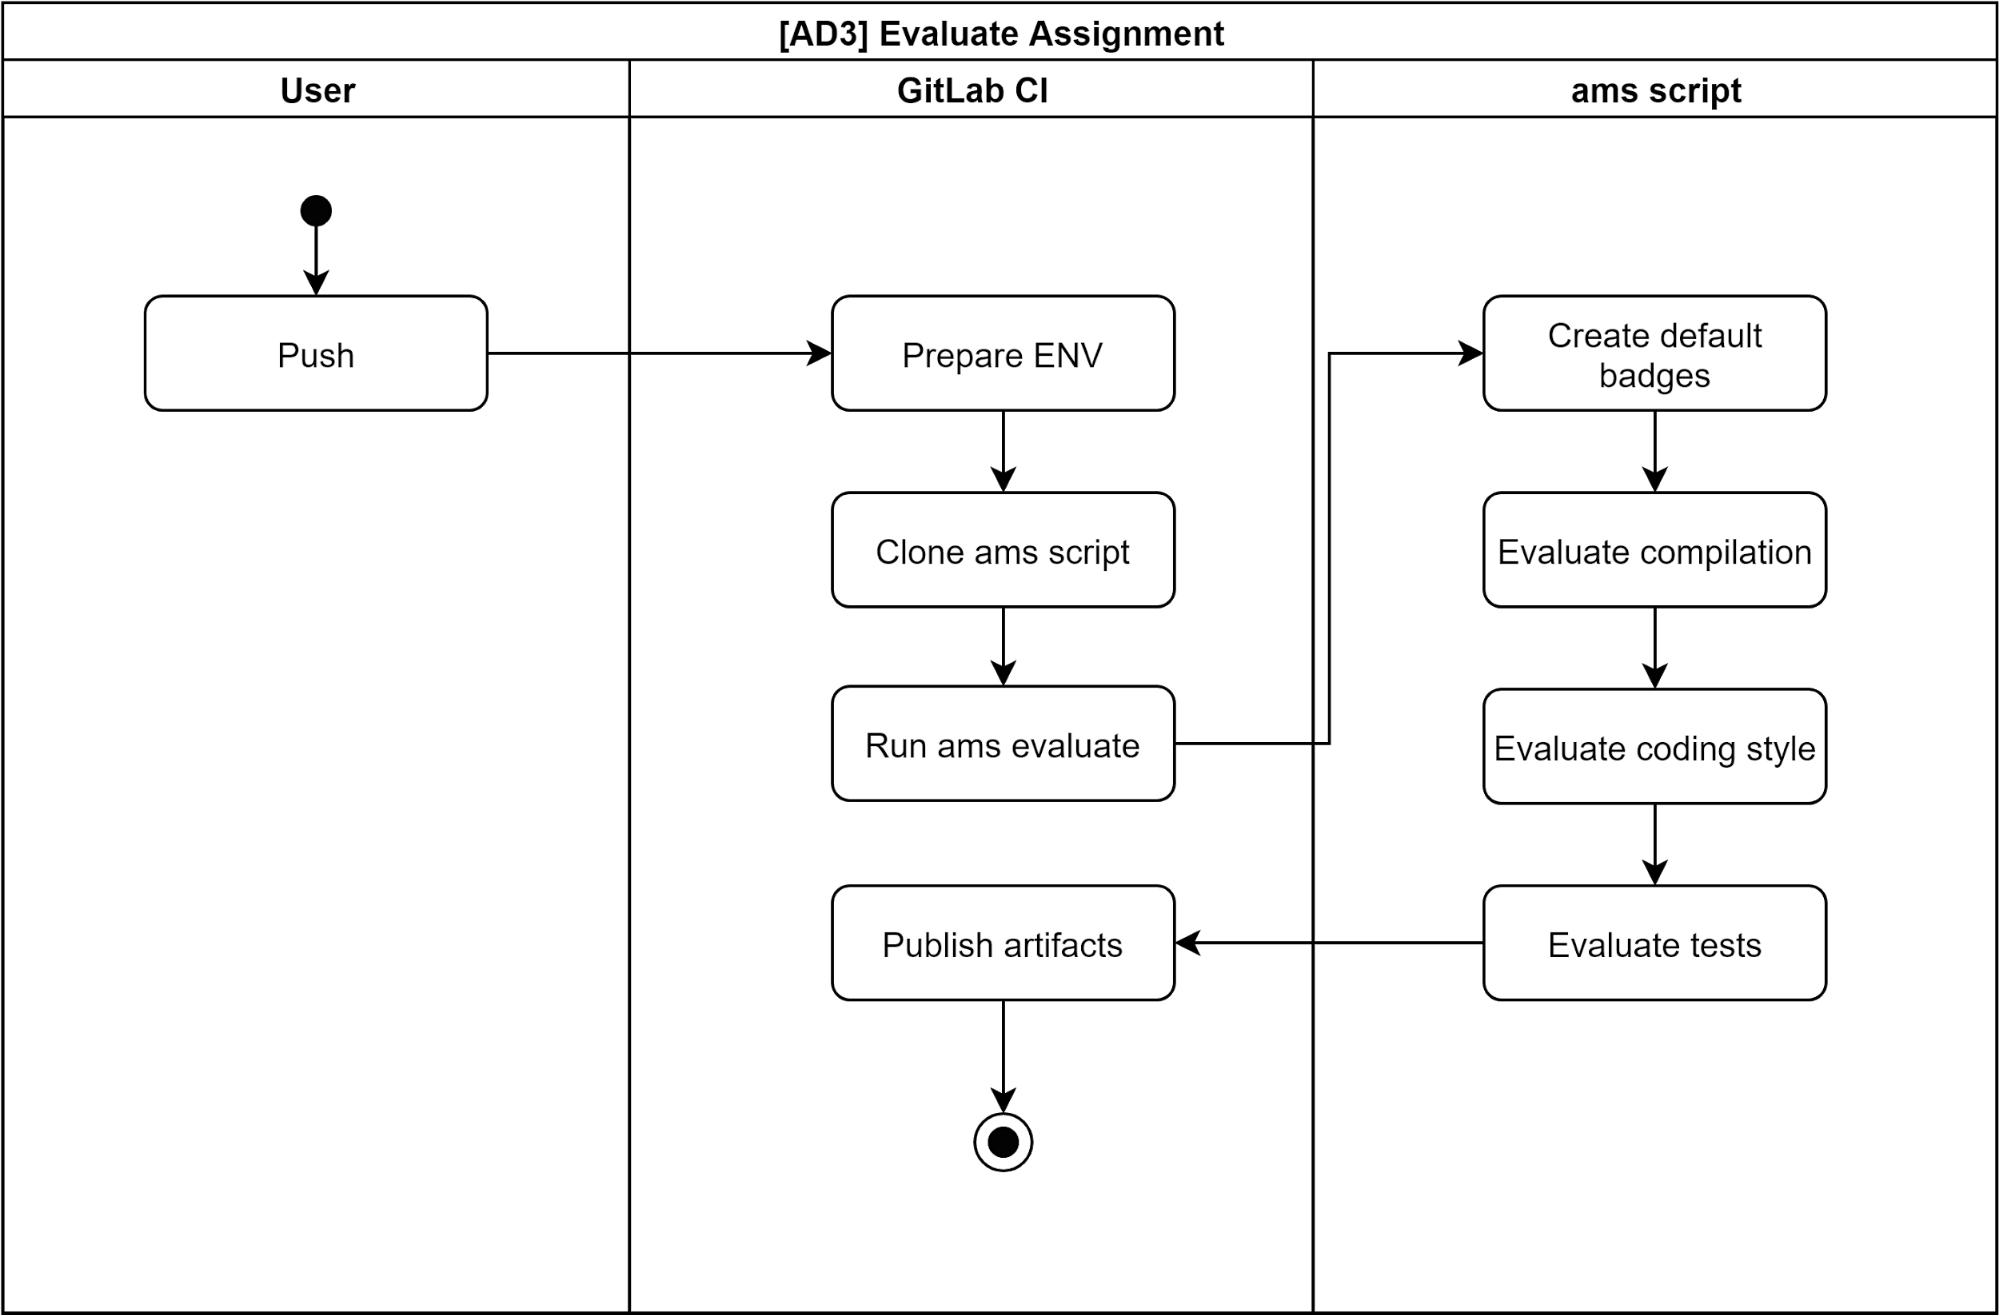
\includegraphics[width=\textwidth,height=\textheight,keepaspectratio]{Figures/ad/ad13.png}
    \caption{Evaluate Assignment activity diagram}
\end{figure}

\subsection{{[}AD4{]} Similarity measure} \label{ssec:ad4}

\begin{figure}[H]
    \centering
    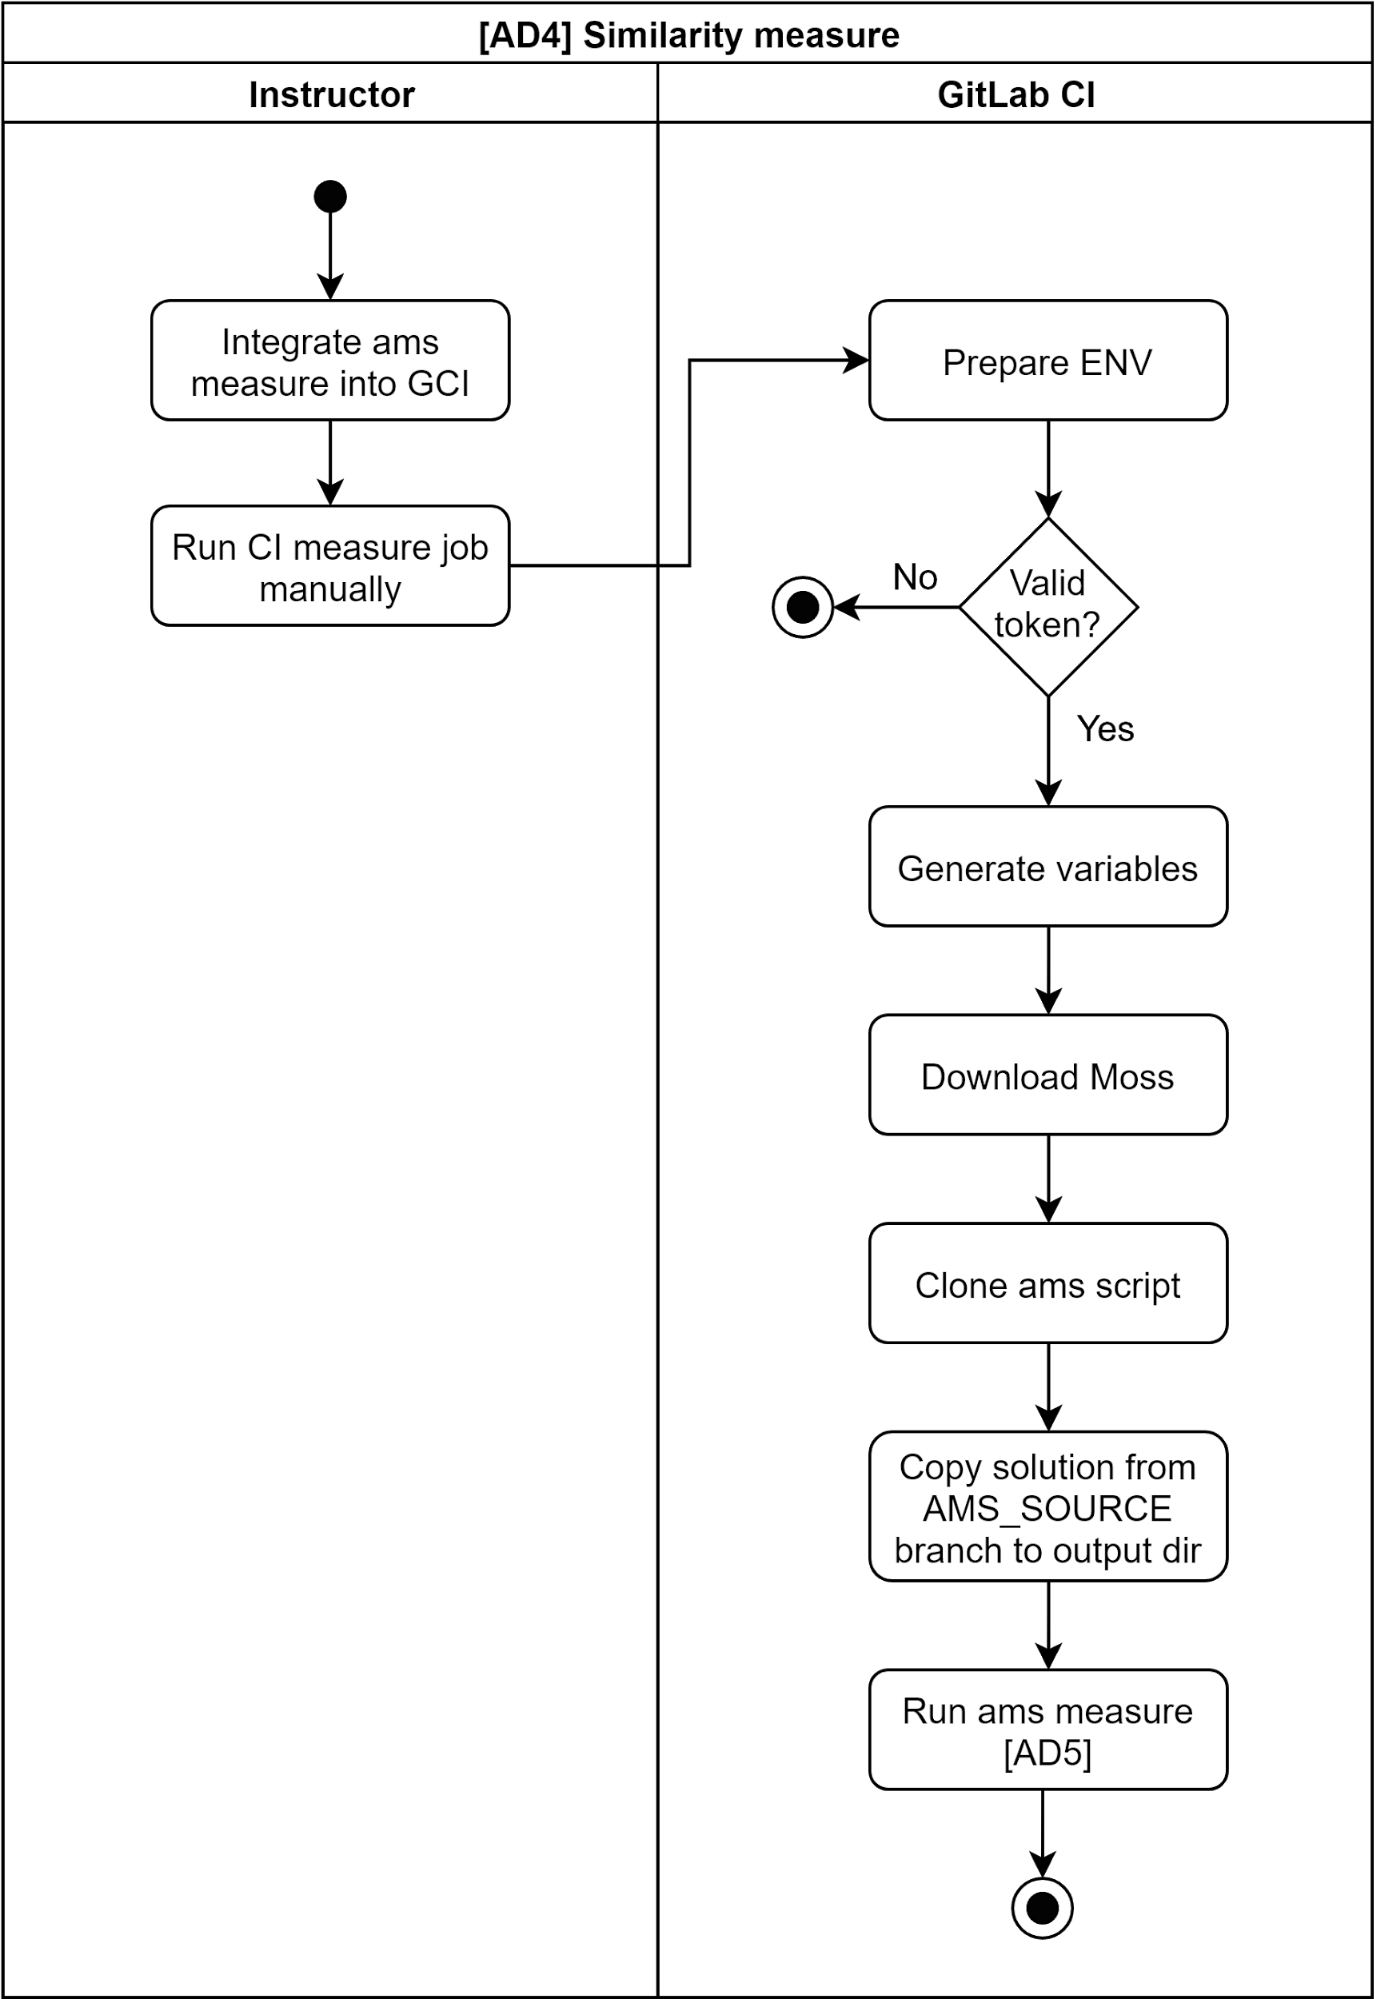
\includegraphics[width=0.8\textwidth,height=\textheight,keepaspectratio]{Figures/ad/ad11.png}
    \caption{Similarity measure activity diagram}
\end{figure}

\subsection{{[}AD5{]} AMS measure} \label{ssec:ad5}

\begin{figure}[H]
    \centering
    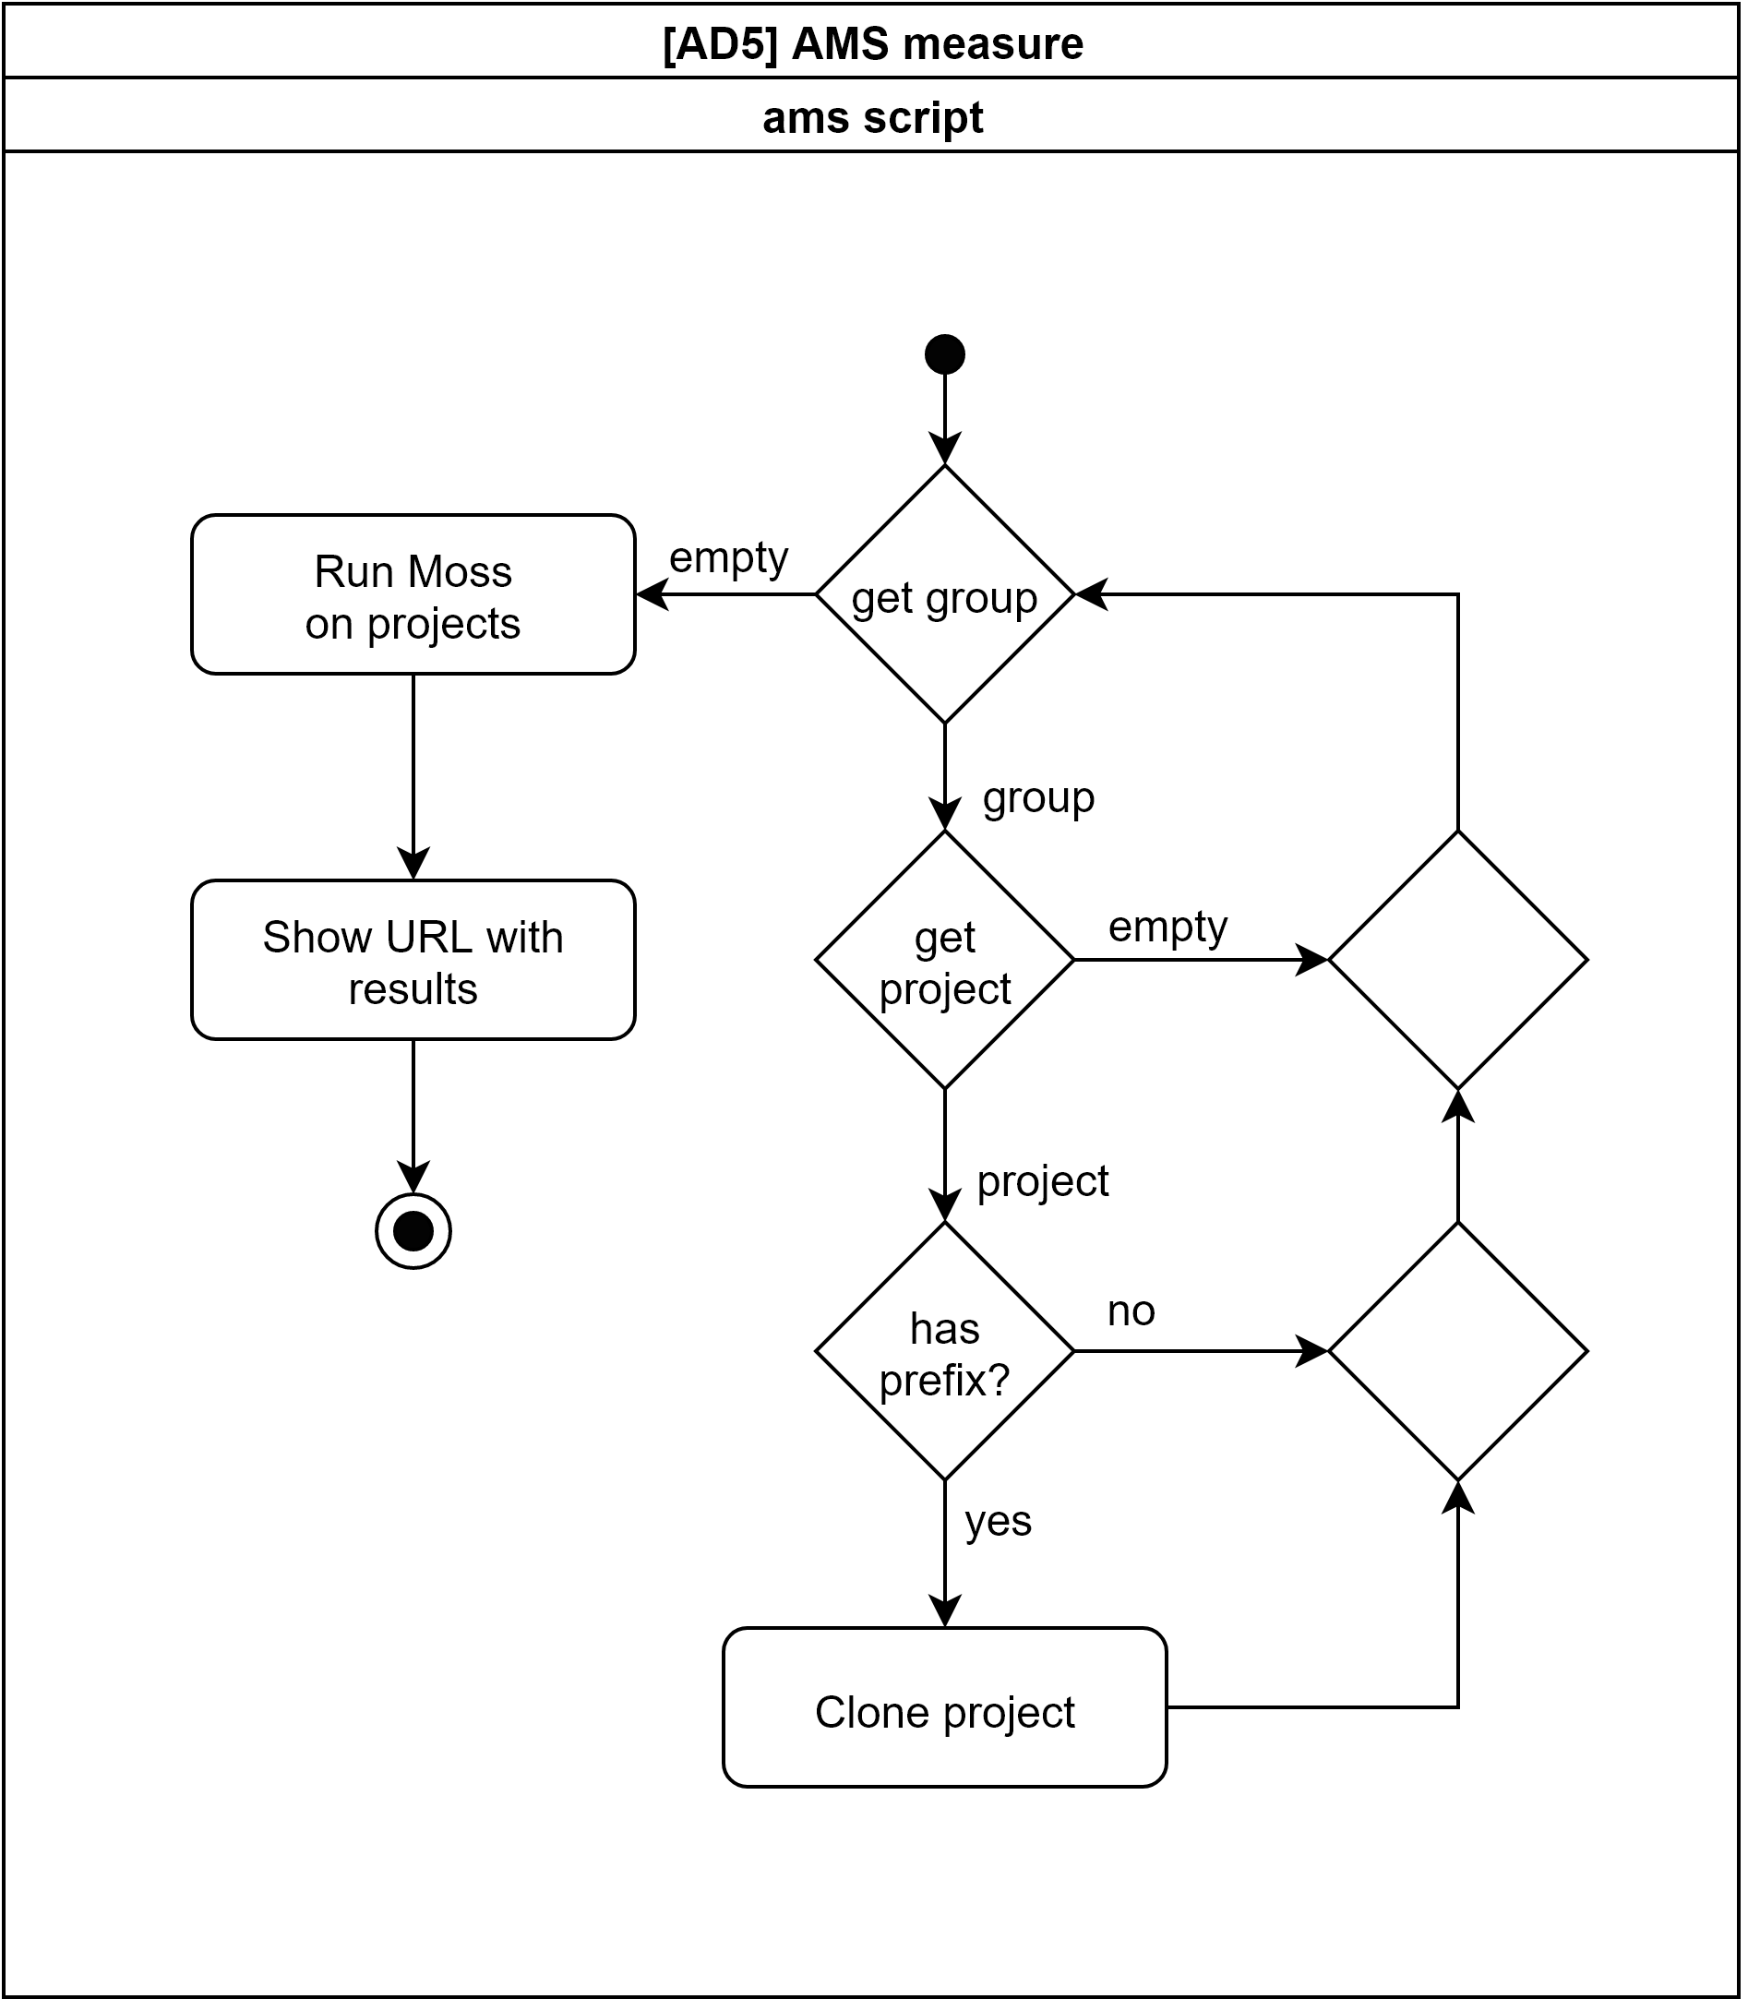
\includegraphics[width=0.8\textwidth,height=\textheight,keepaspectratio]{Figures/ad/ad17.png}
    \caption{AMS measure activity diagram}
\end{figure}

\subsection{{[}AD6{]} Collective evaluation} \label{ssec:ad6}

\begin{figure}[H]
    \centering
    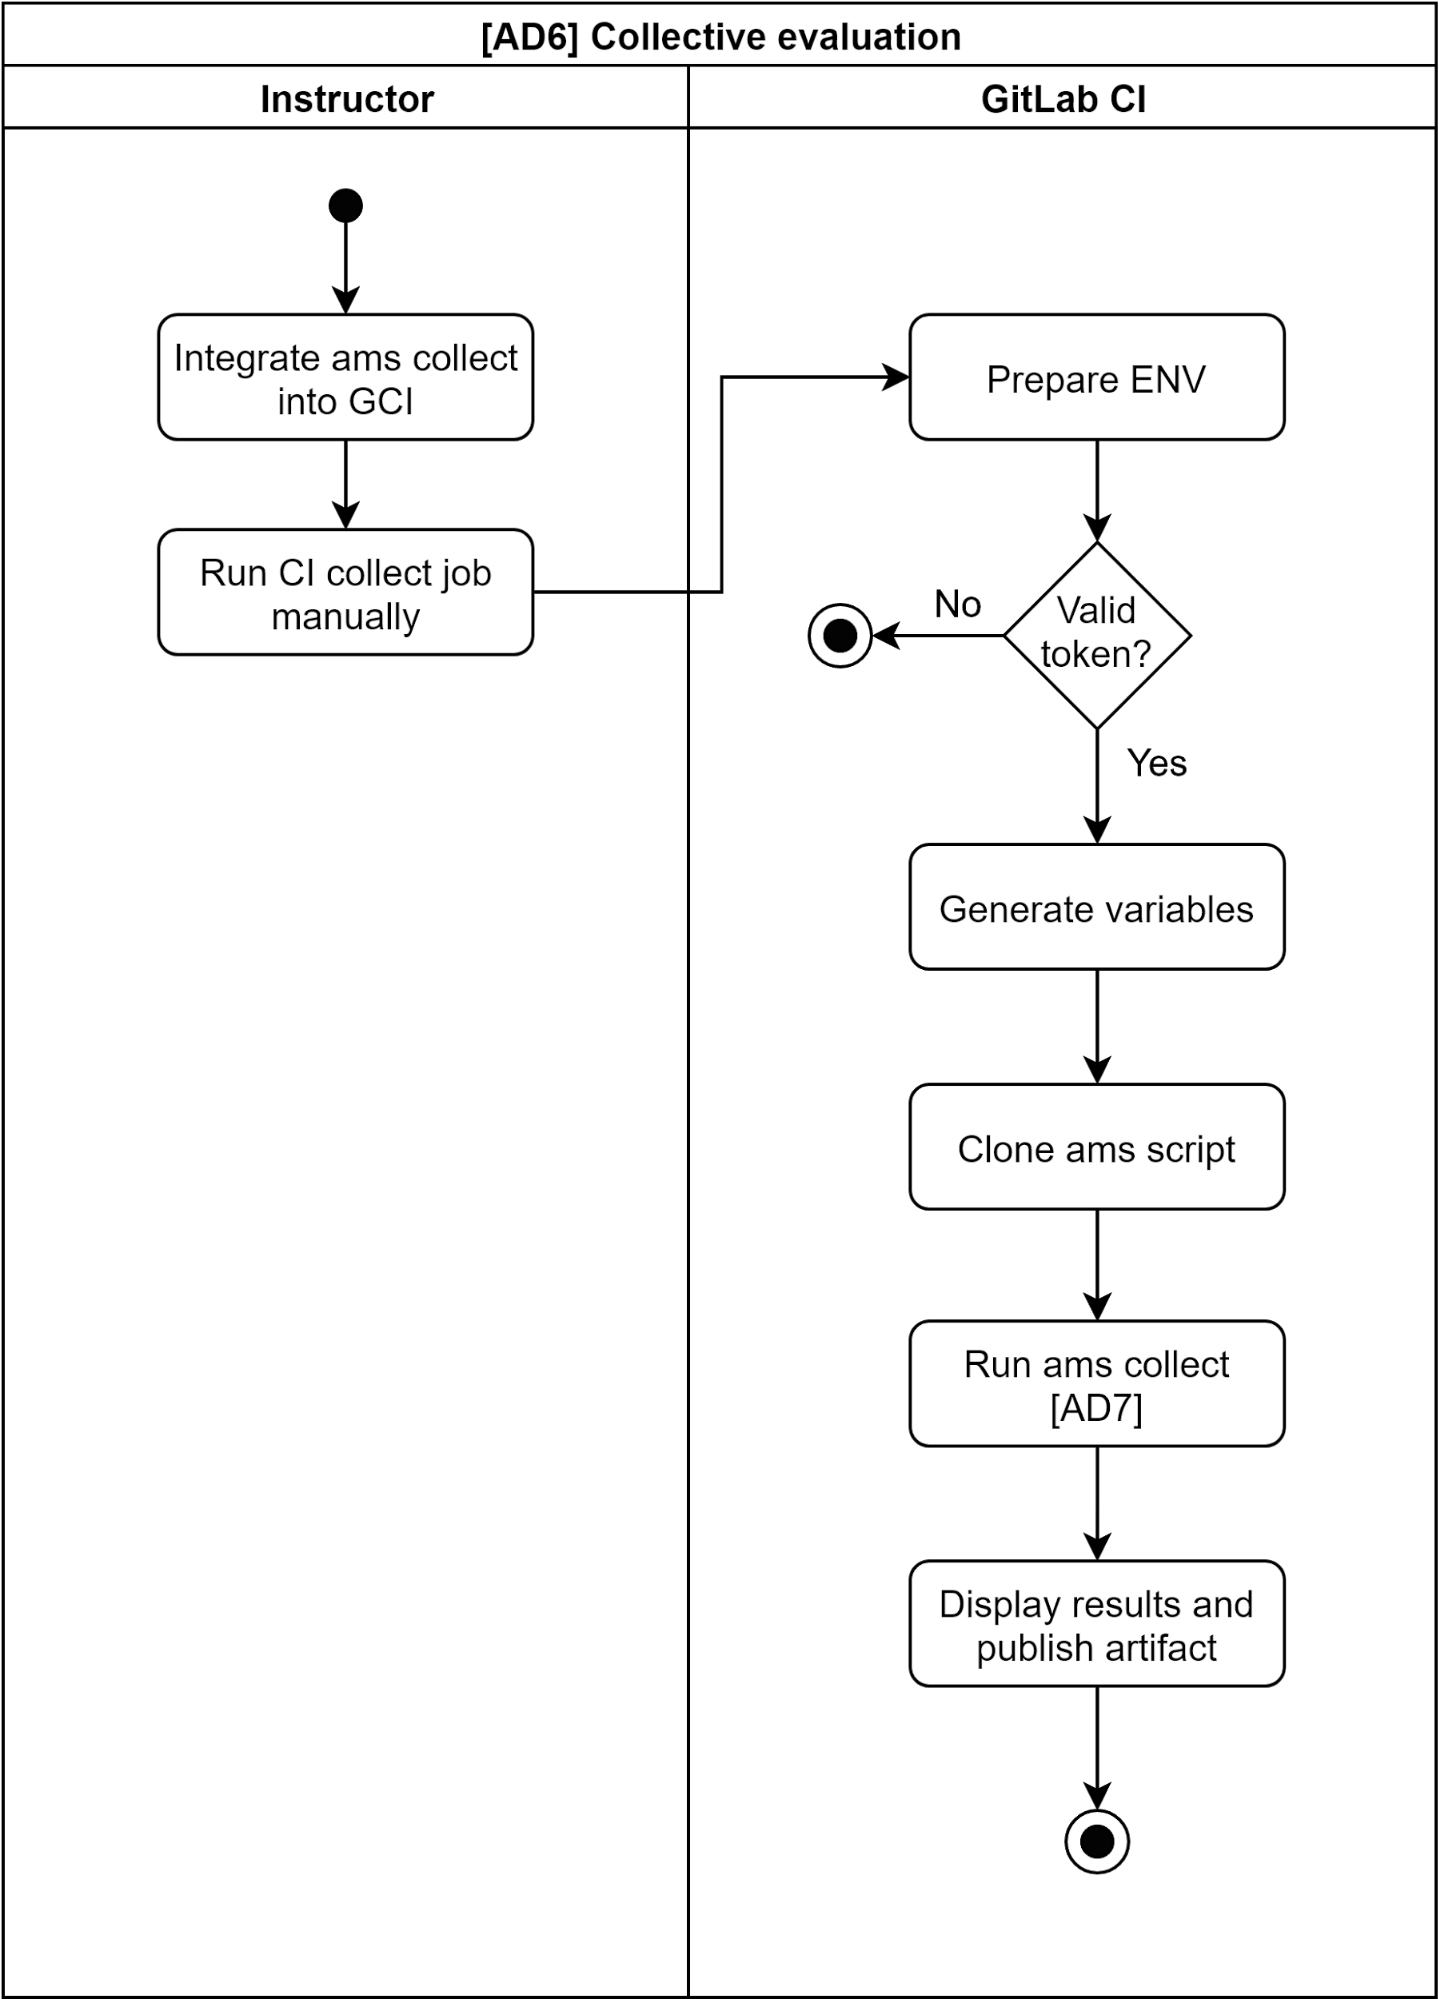
\includegraphics[width=0.8\textwidth,height=\textheight,keepaspectratio]{Figures/ad/ad12.png}
    \caption{Collective evaluation activity diagram}
\end{figure}

\subsection{{[}AD7{]} AMS collect} \label{ssec:ad7}

\begin{figure}[H]
    \centering
    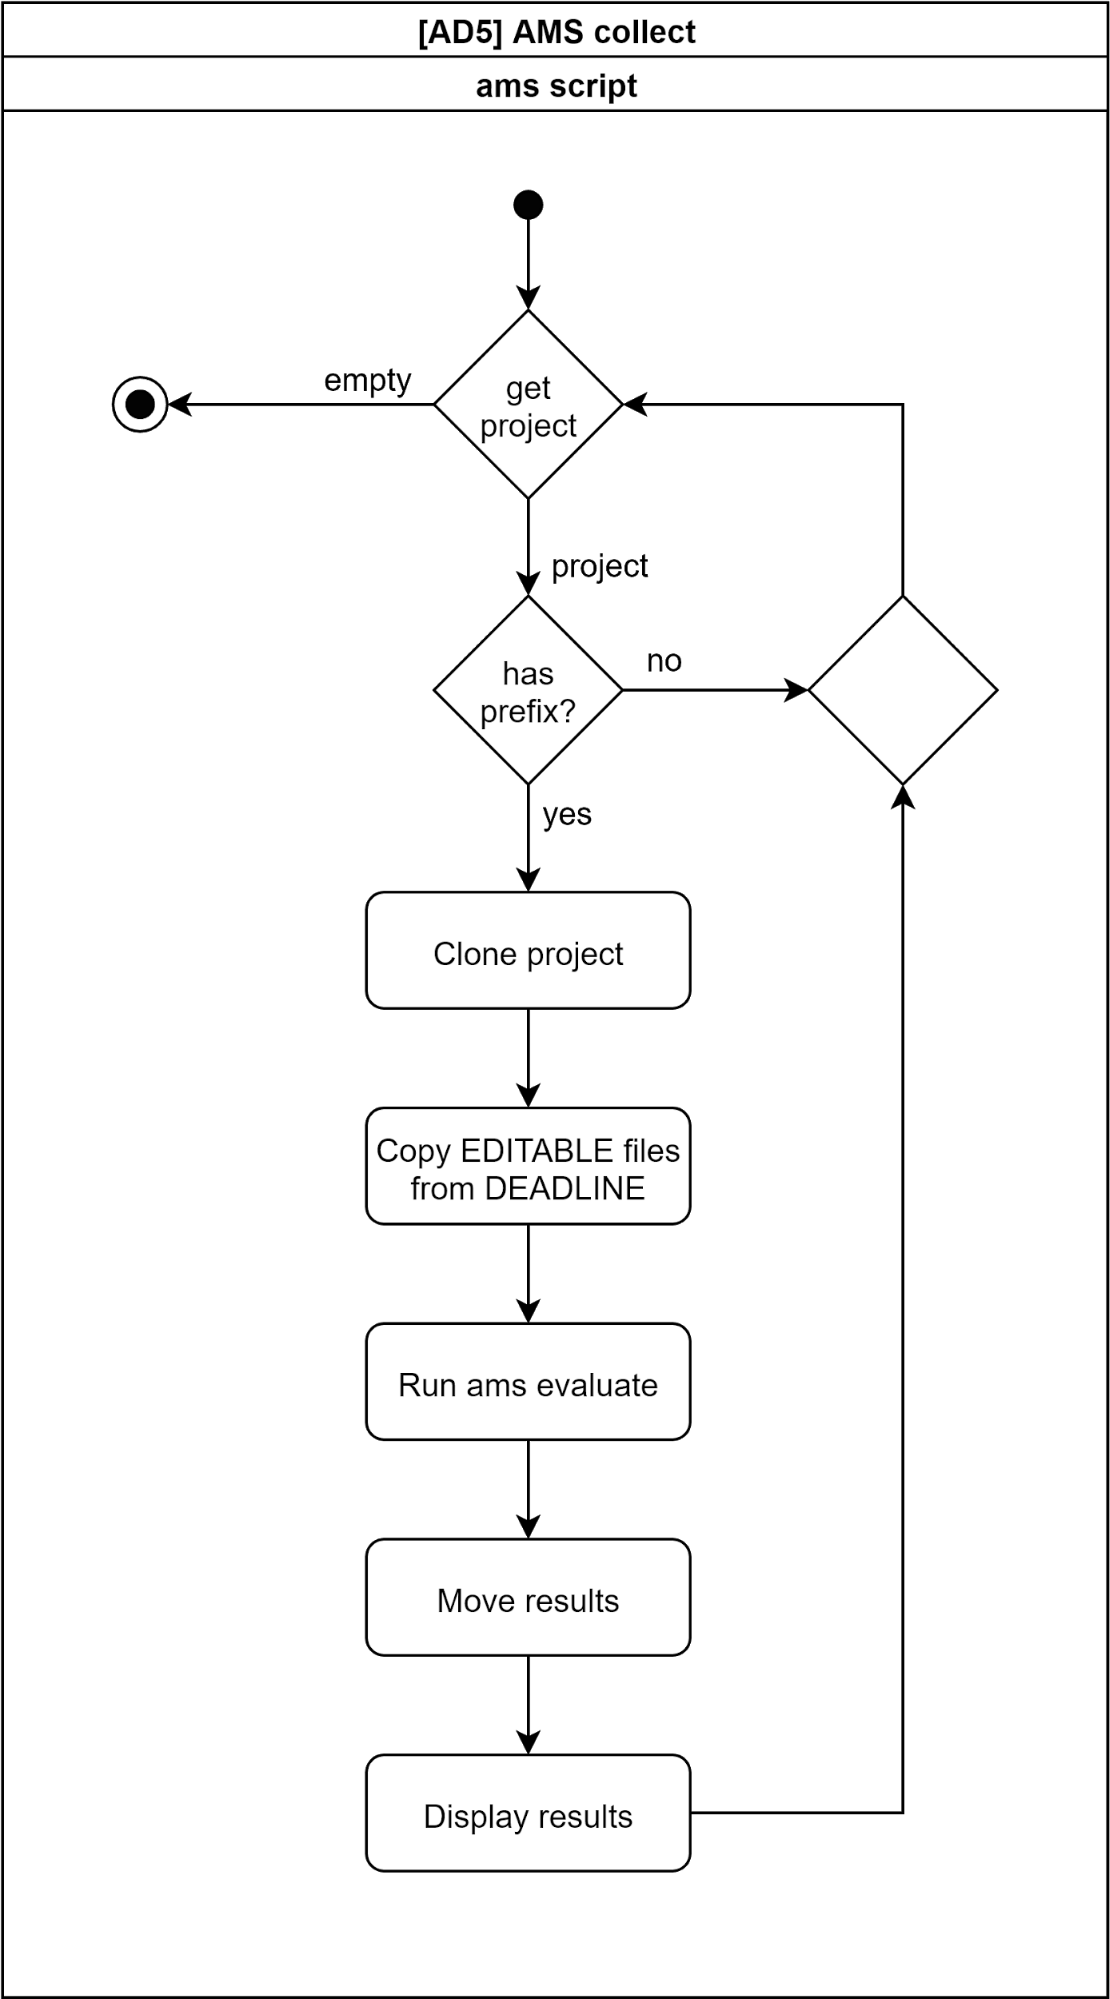
\includegraphics[width=\textwidth,height=.85\textheight,keepaspectratio]{Figures/ad/ad7.png}
    \caption{AMS collect activity diagram}
\end{figure}

\subsection{{[}AD8{]} Create new GitLab working project} \label{ssec:ad8}

\begin{figure}[H]
    \centering
    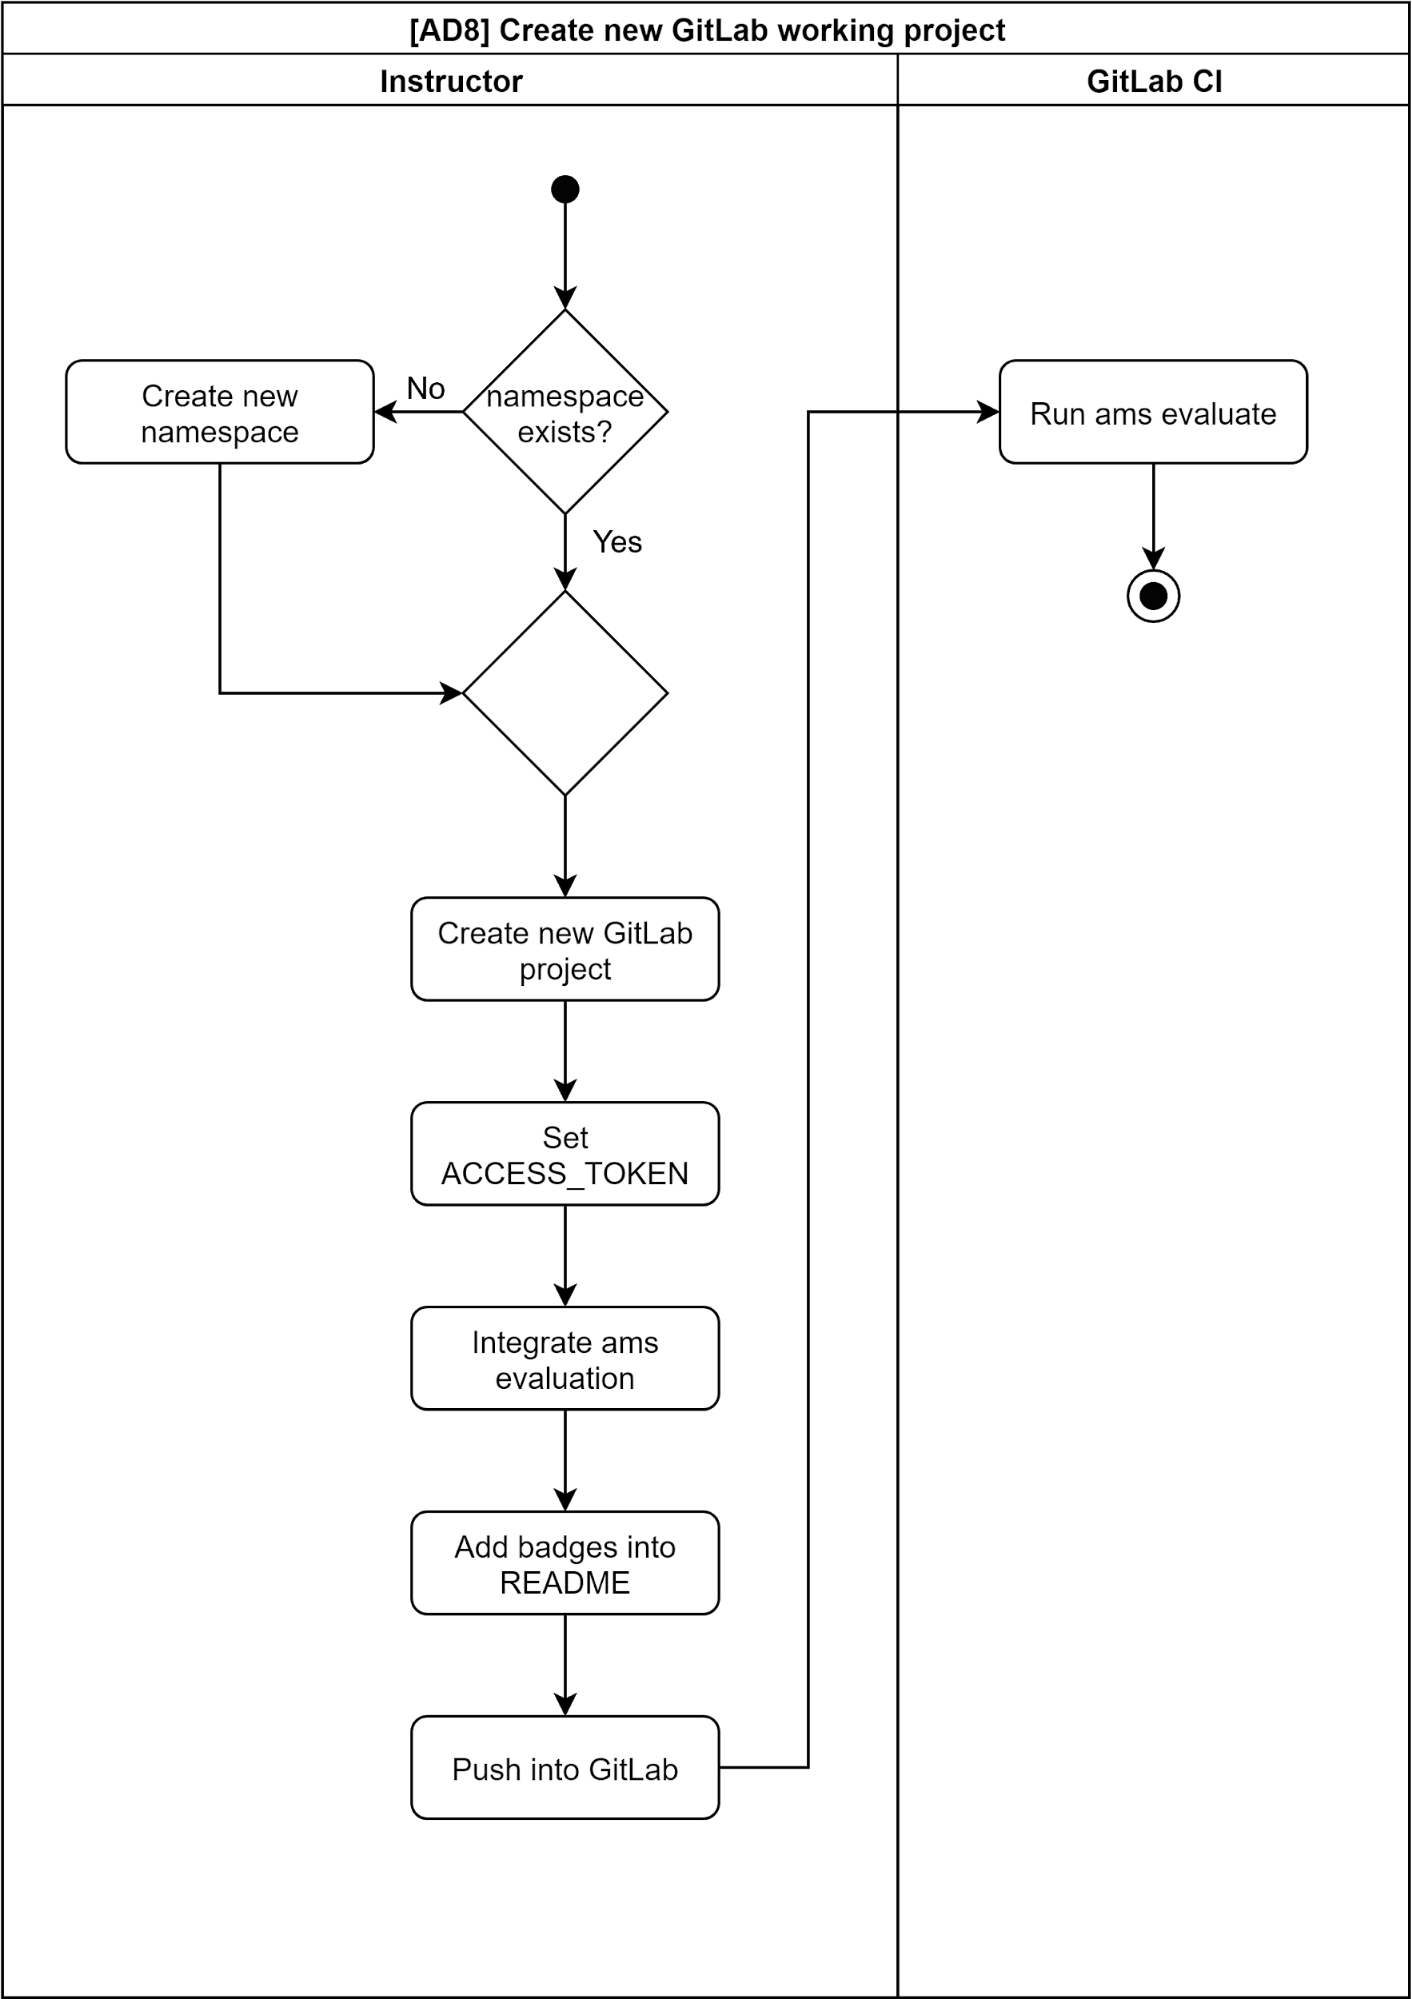
\includegraphics[width=\textwidth,height=.85\textheight,keepaspectratio]{Figures/ad/ad8.png}
    \caption{Create new GitLab working project activity diagram}
\end{figure}

\subsection{{[}AD9{]} Create an assignment from the working project} \label{ssec:ad9}

\begin{figure}[H]
    \centering
    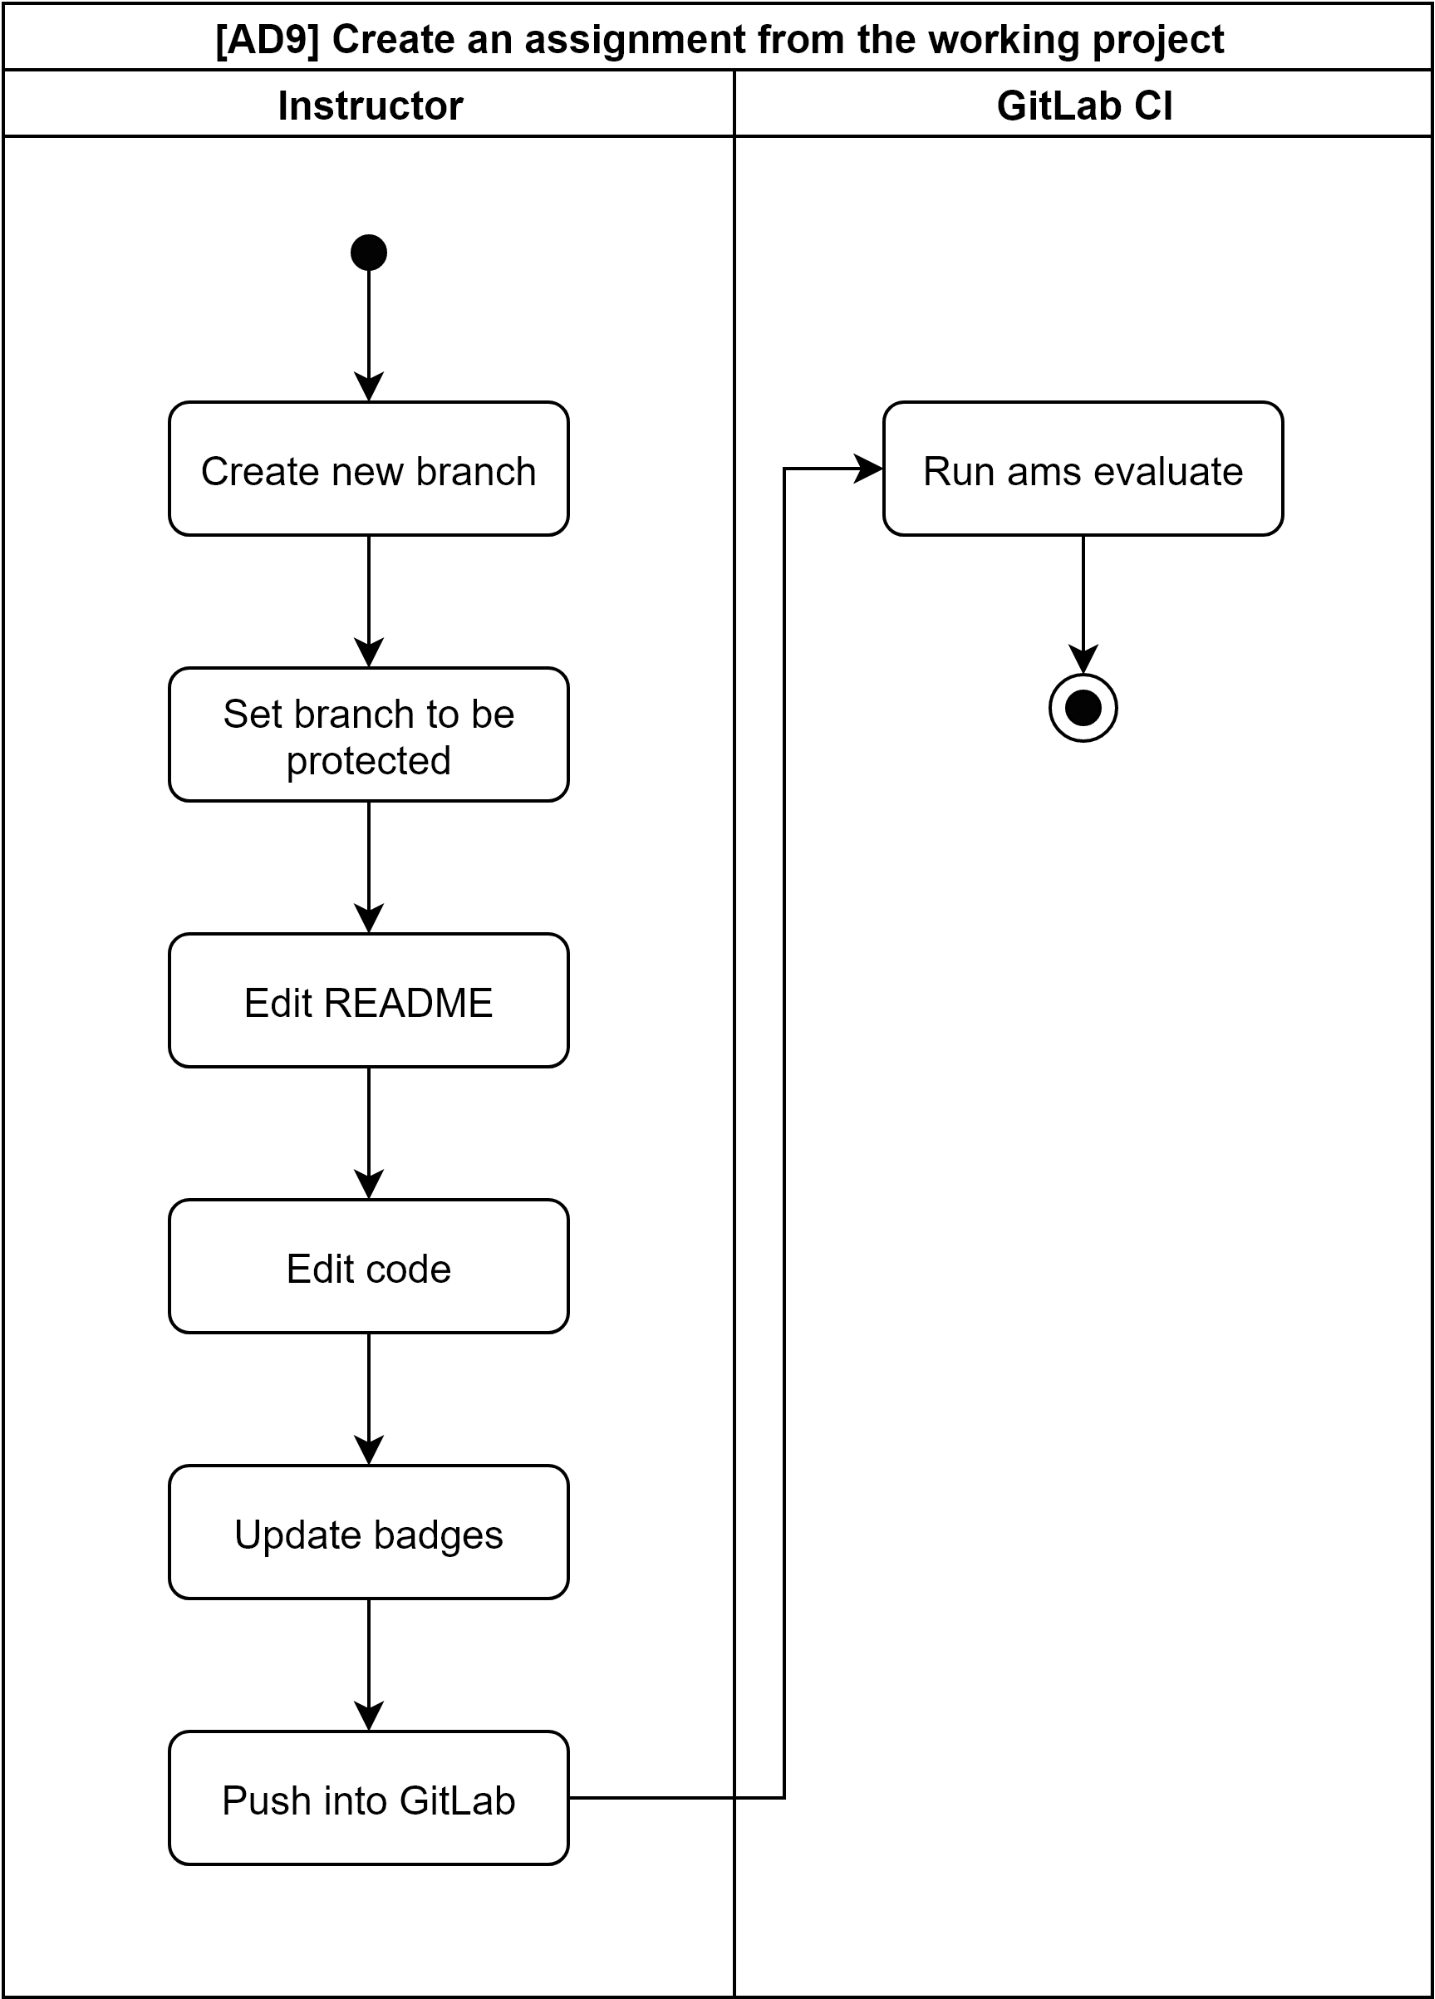
\includegraphics[width=0.8\textwidth,height=\textheight,keepaspectratio]{Figures/ad/ad2.png}
    \caption{Create an assignment from the working project activity diagram}
\end{figure}

\subsection{{[}AD10{]} Providing remote support} \label{ssec:ad10}

\begin{figure}[H]
    \centering
    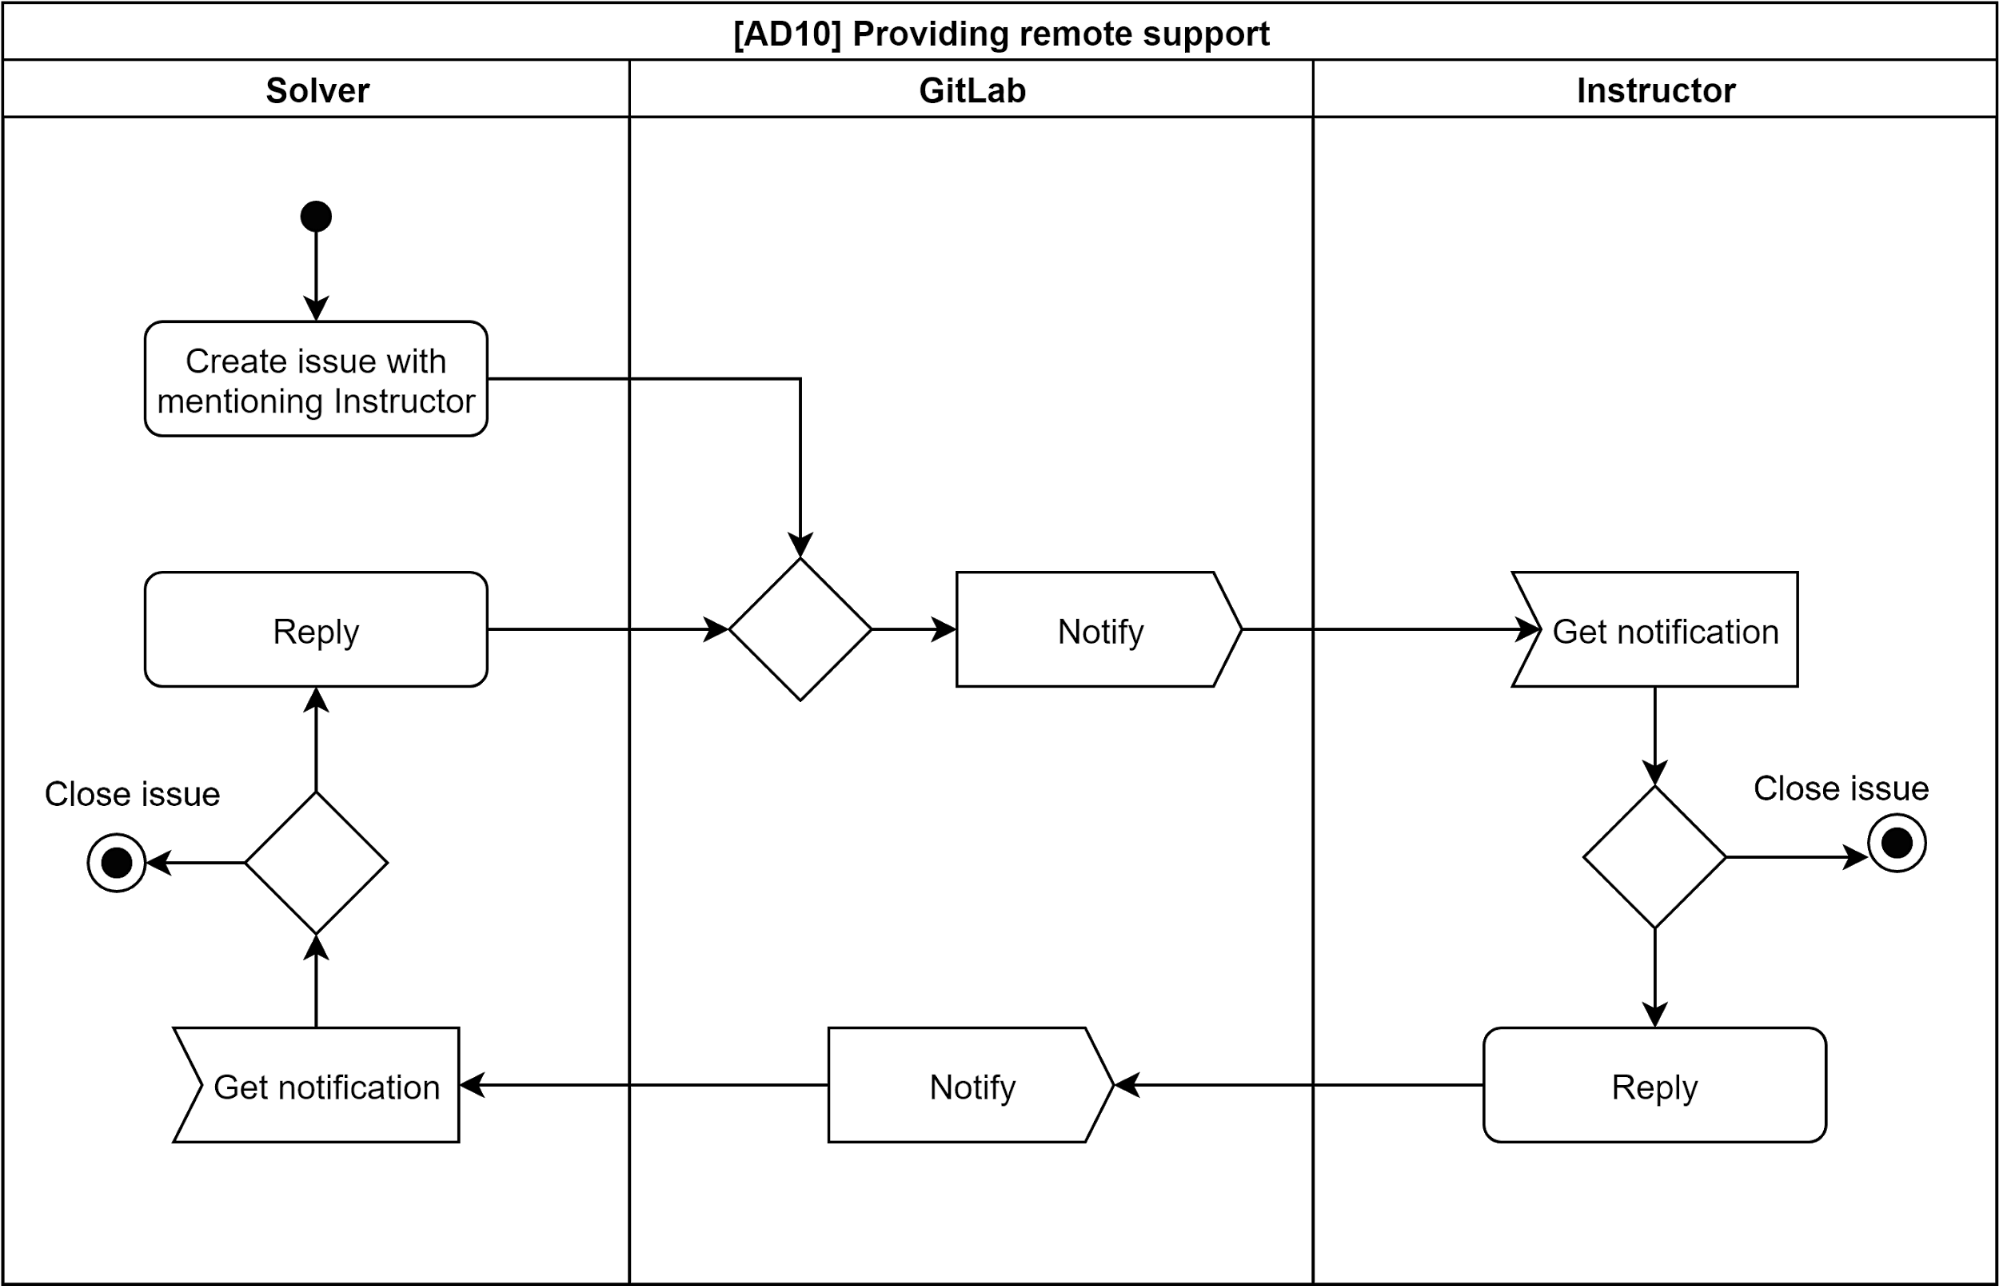
\includegraphics[width=\textwidth,height=\textheight,keepaspectratio]{Figures/ad/ad14.png}
    \caption{Providing remote support activity diagram}
\end{figure}

\subsection{{[}AD11{]} Merge update into solver assignment} \label{ssec:ad11}

\begin{figure}[H]
    \centering
    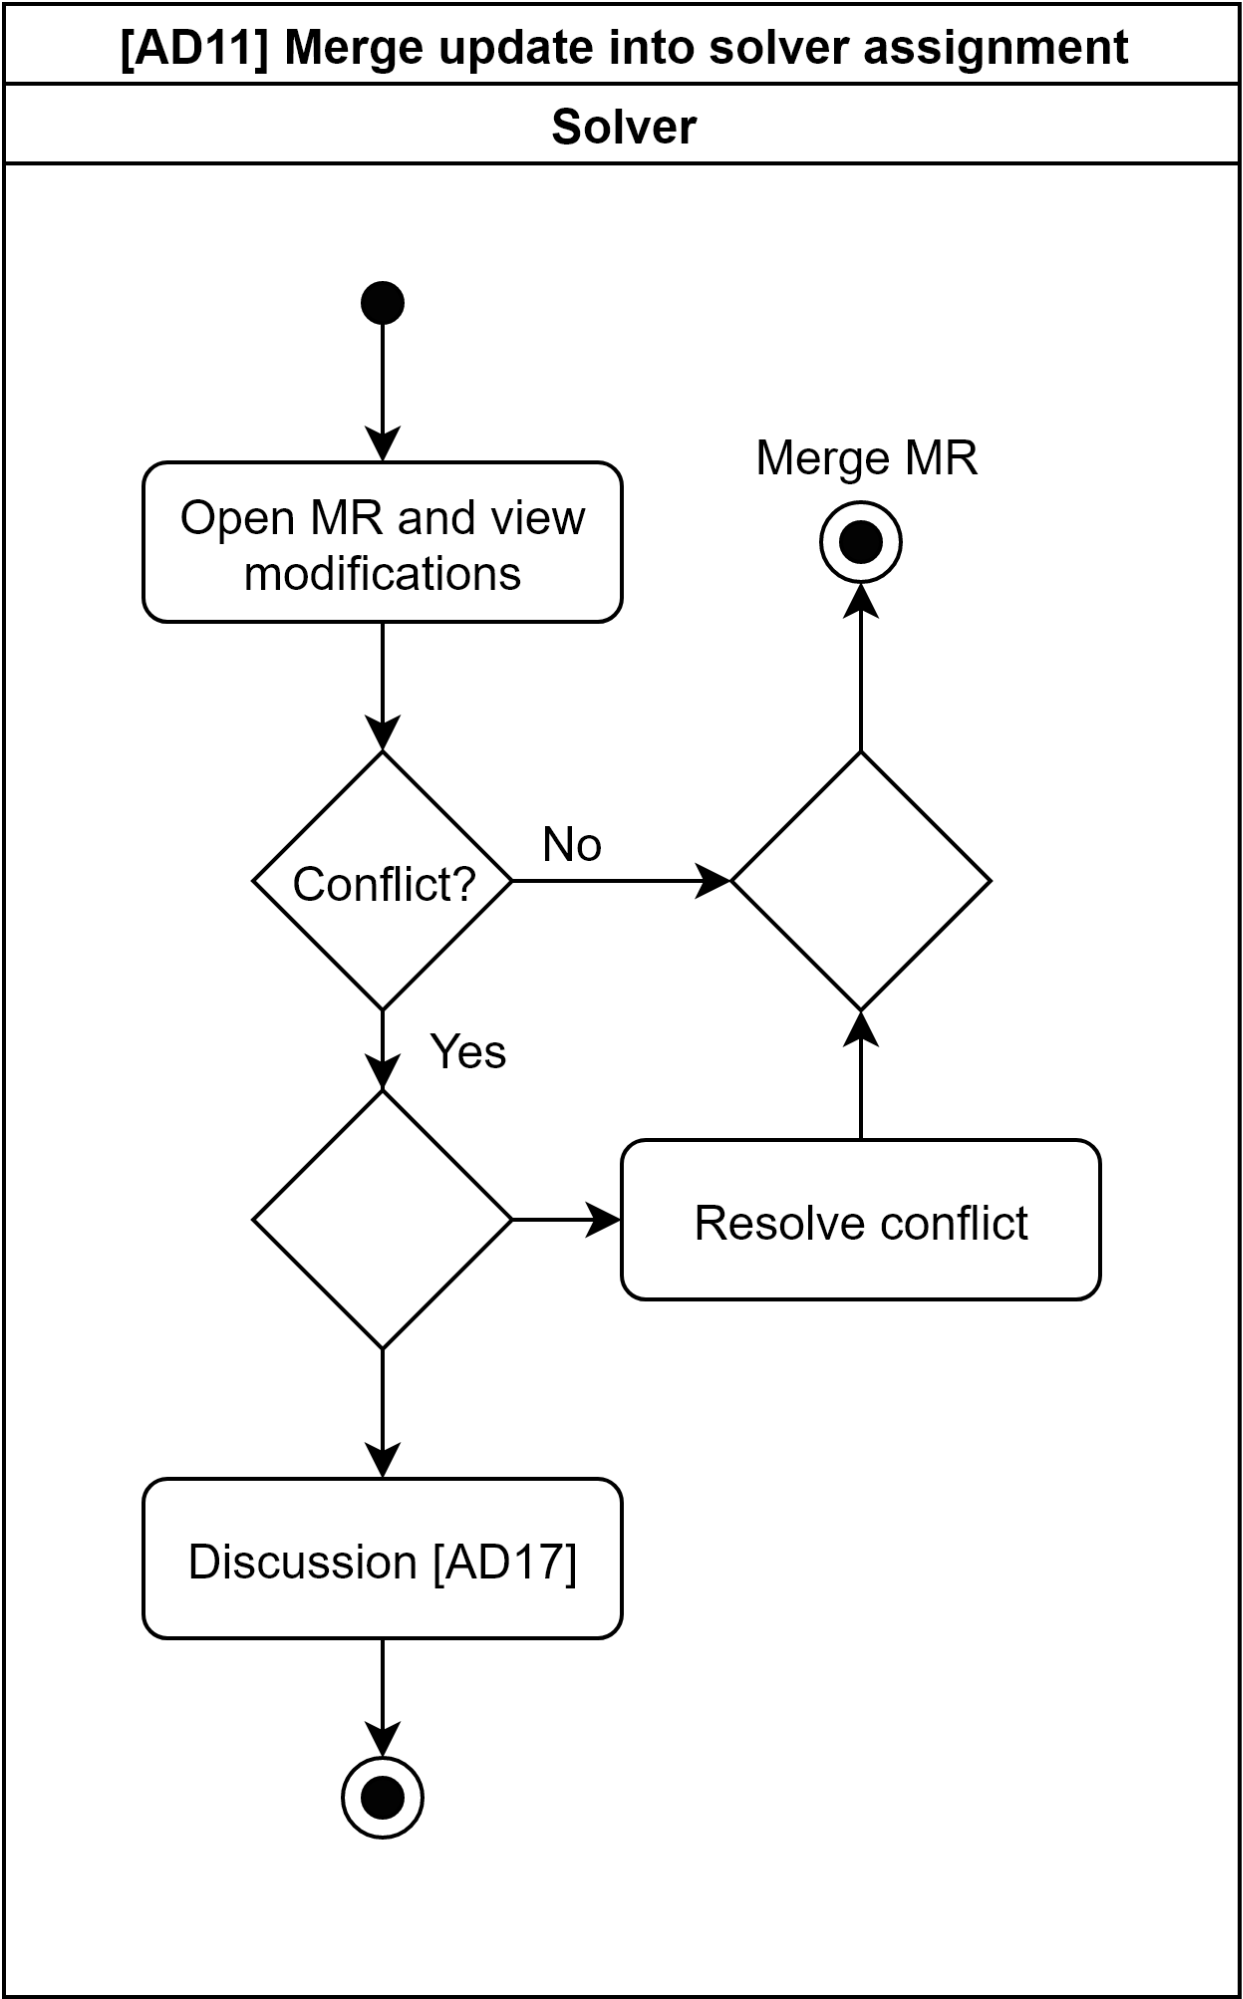
\includegraphics[width=0.6\textwidth,height=\textheight,keepaspectratio]{Figures/ad/ad9.png}
    \caption{Merge update into solver assignment activity diagram}
\end{figure}

\subsection{{[}AD12{]} Edit assignment online} \label{ssec:ad12}

\begin{figure}[H]
    \centering
    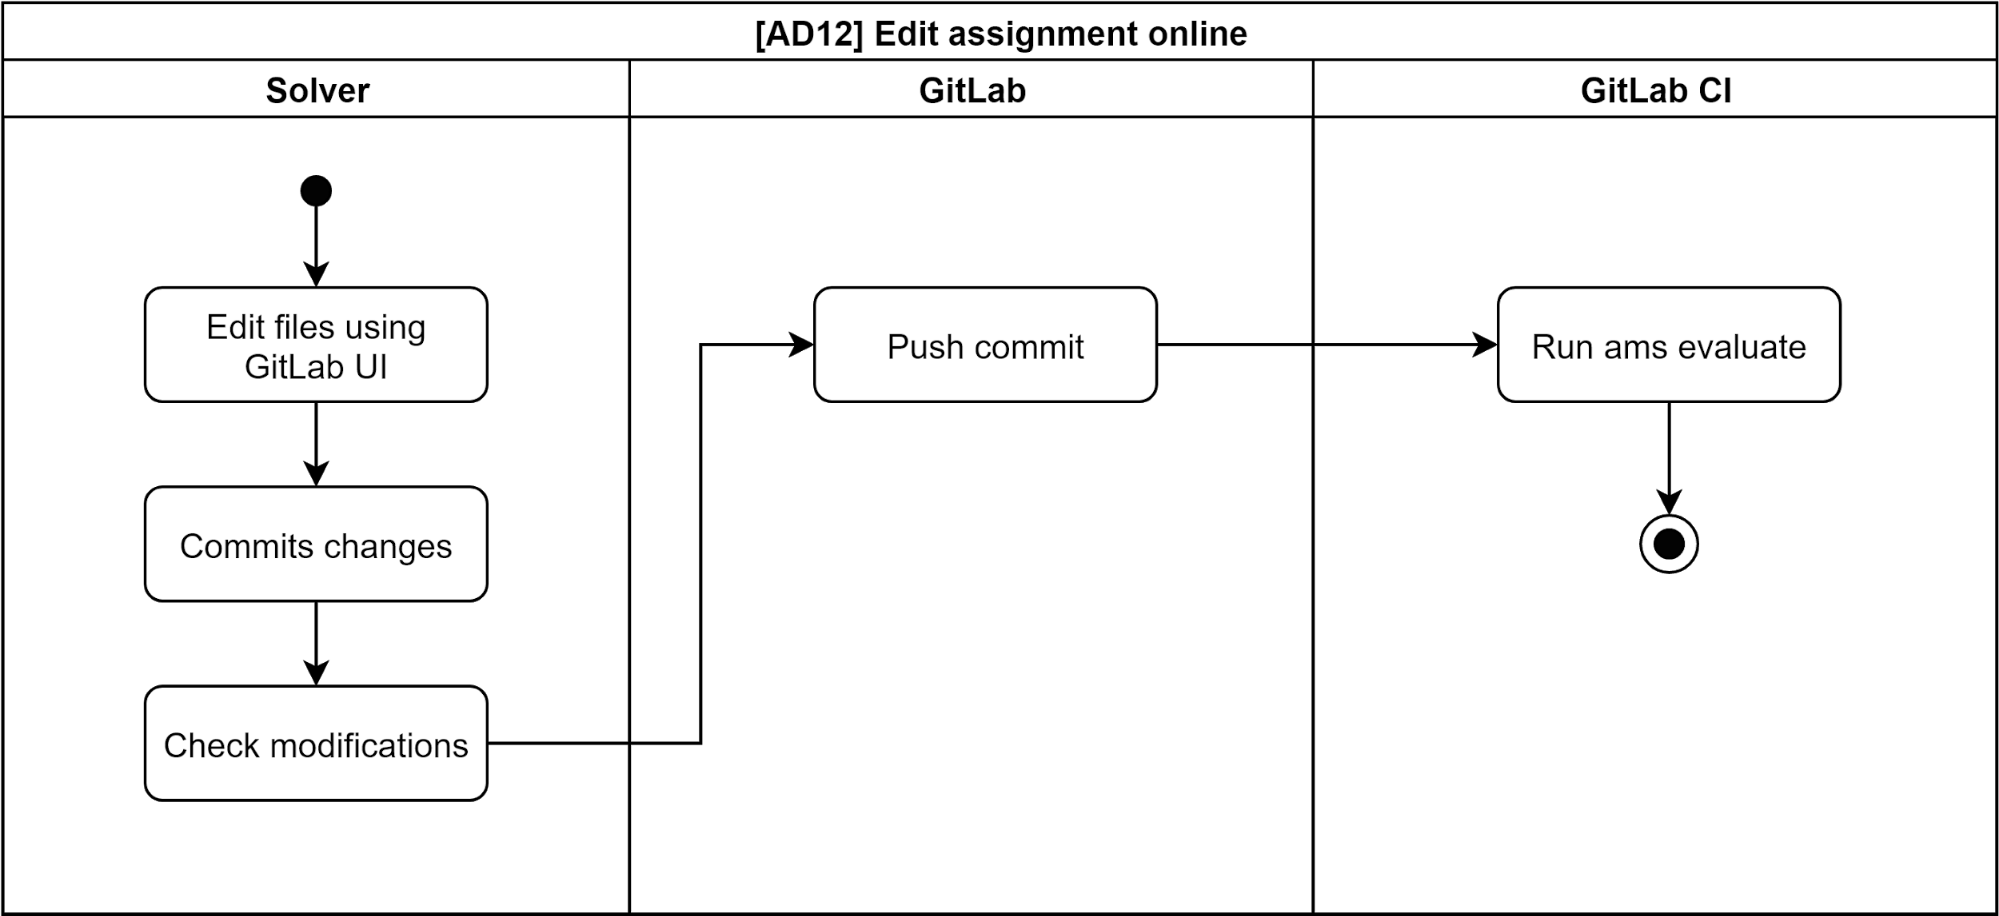
\includegraphics[width=\textwidth,height=\textheight,keepaspectratio]{Figures/ad/ad15.png}
    \caption{Edit assignment online activity diagram}
\end{figure}

\subsection{{[}AD13{]} Edit assignment locally} \label{ssec:ad13}

\begin{figure}[H]
    \centering
    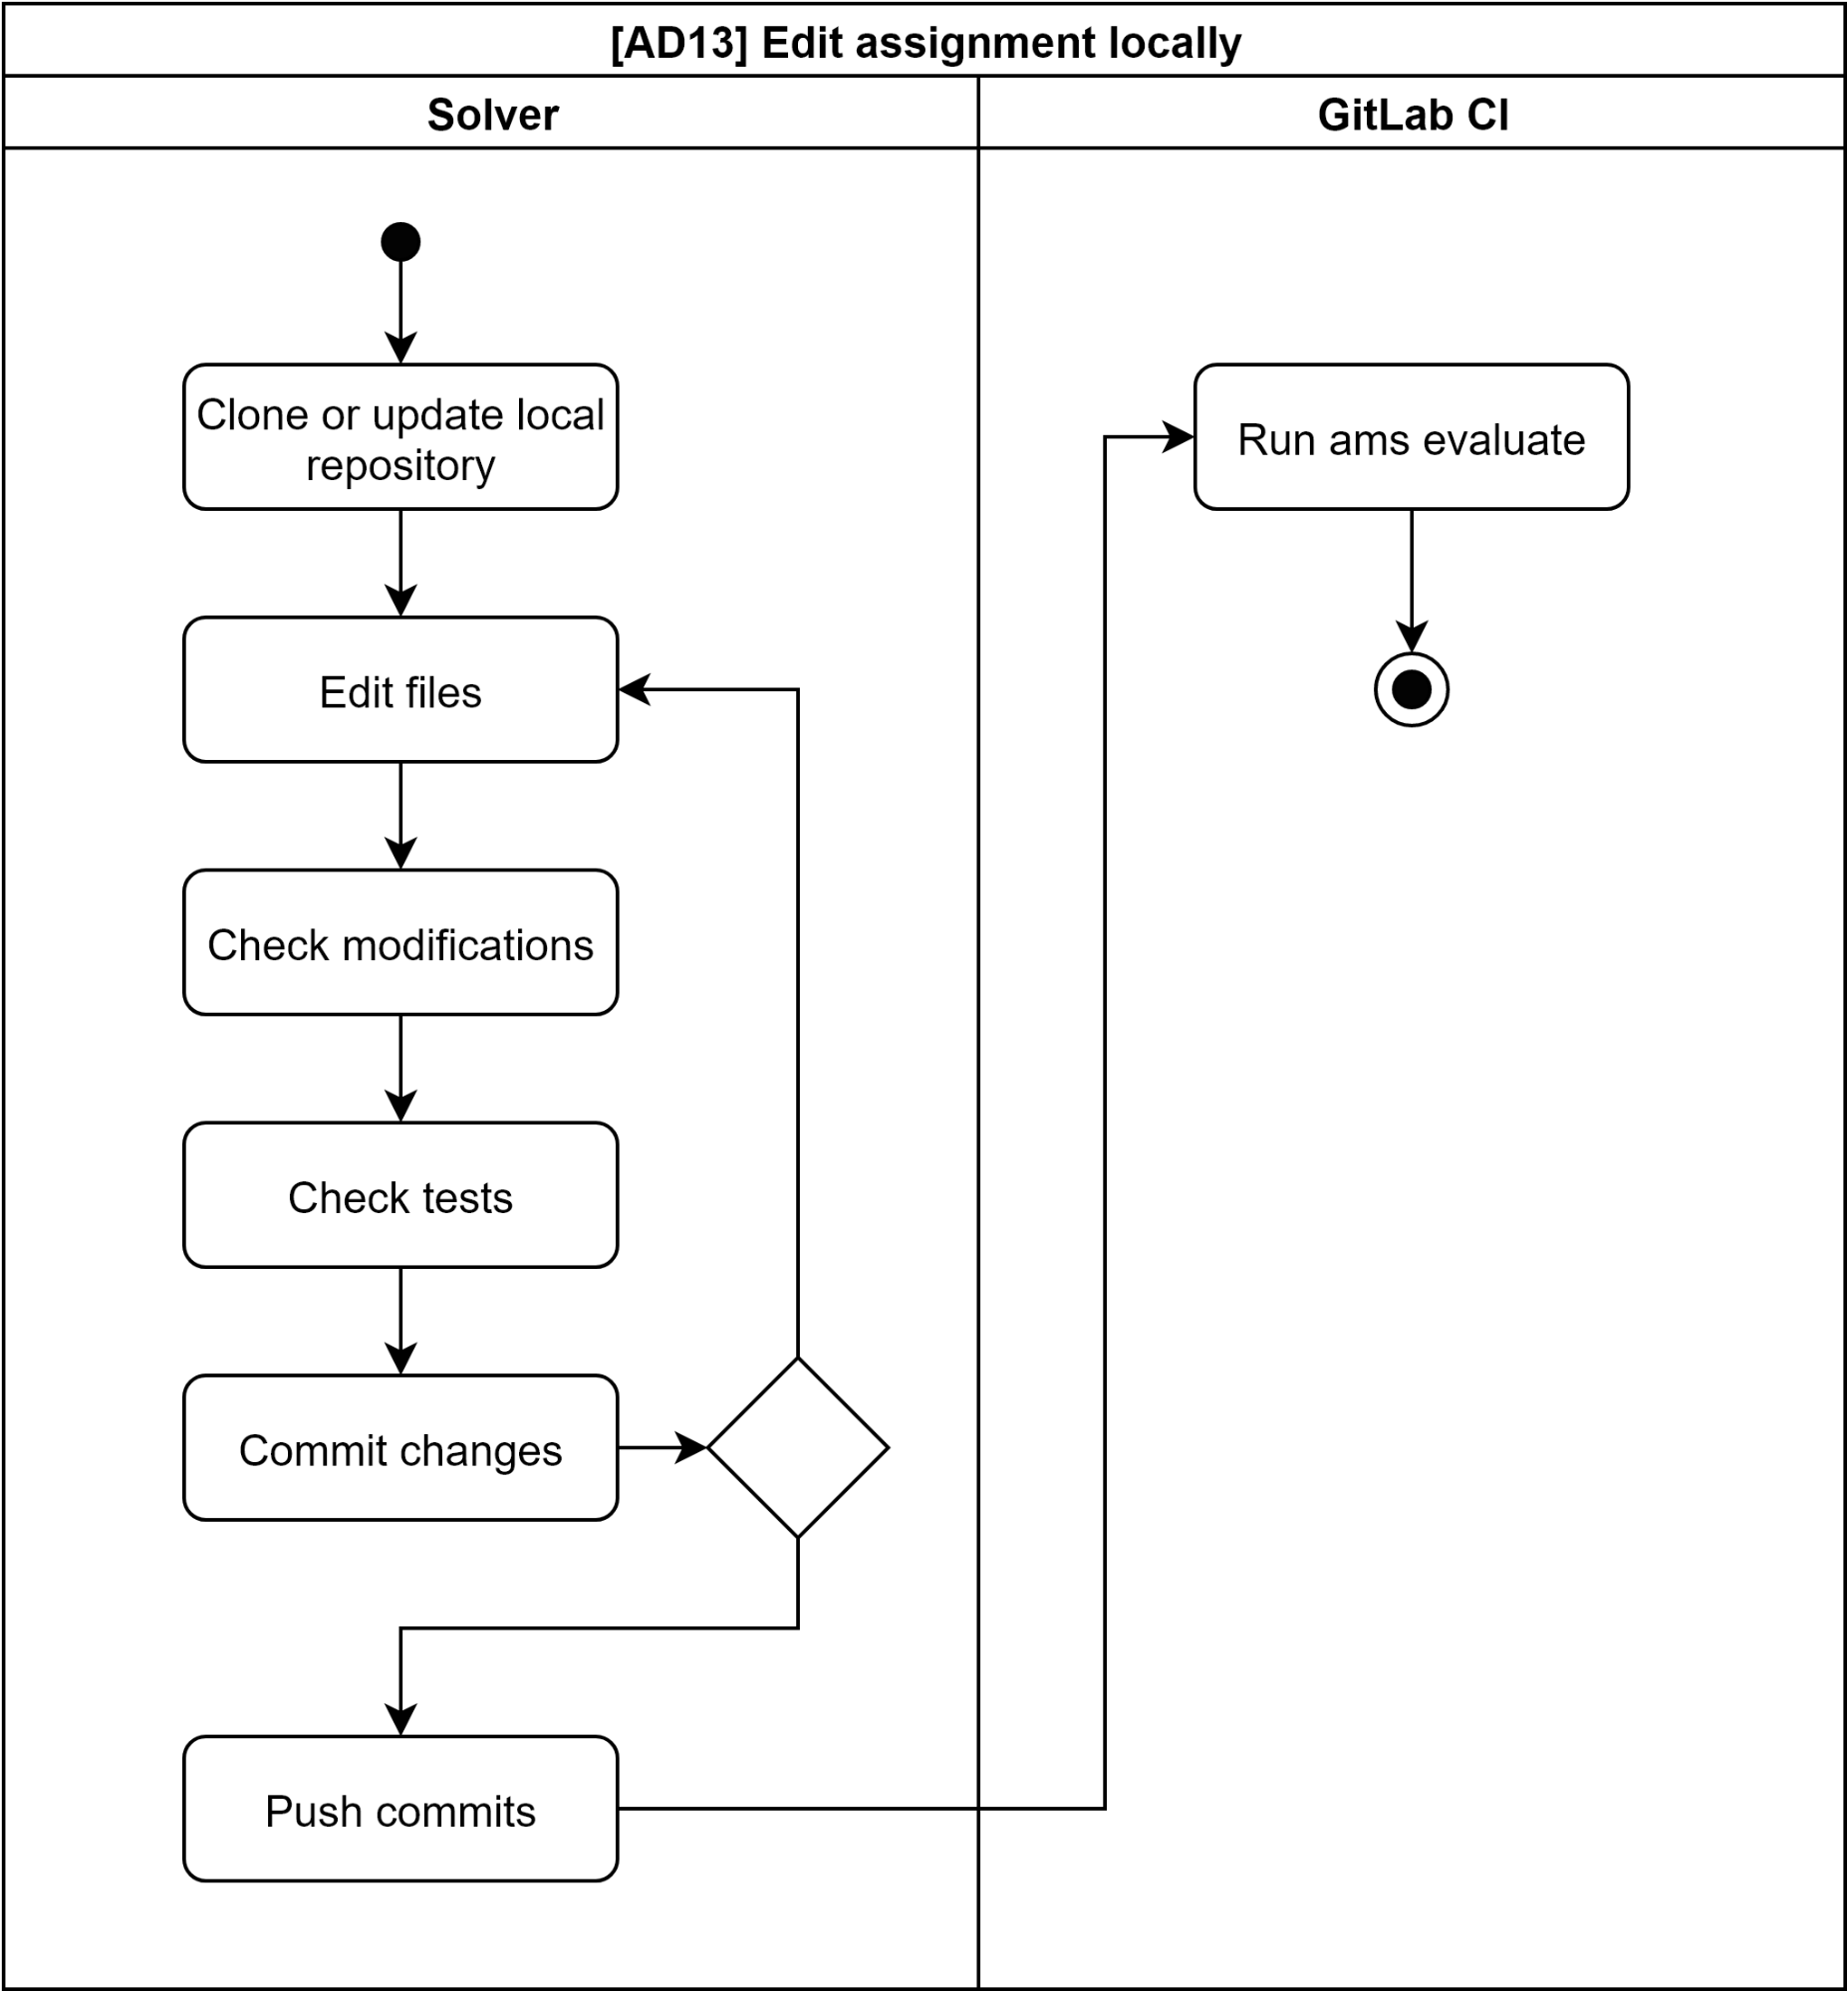
\includegraphics[width=\textwidth,height=\textheight,keepaspectratio]{Figures/ad/ad16.png}
    \caption{Edit assignment locally activity diagram}
\end{figure}

\subsection{{[}AD14{]} View solution diff with working project} \label{ssec:ad14}

\begin{figure}[H]
    \centering
    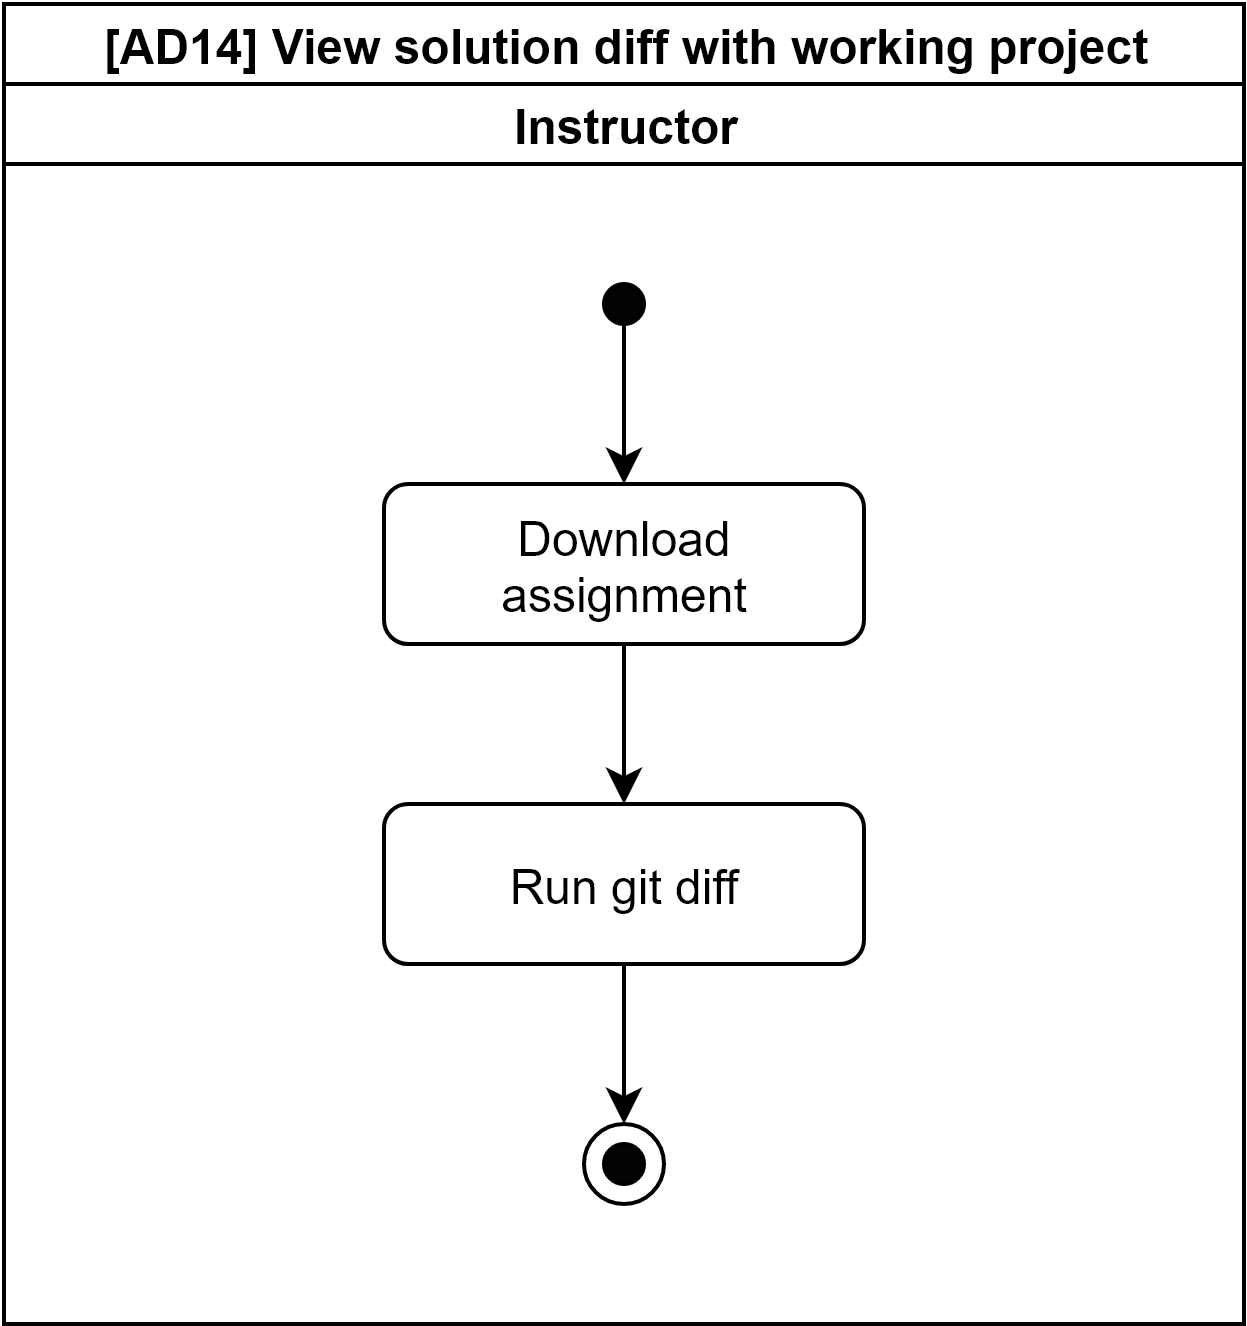
\includegraphics[width=0.6\textwidth,height=\textheight,keepaspectratio]{Figures/ad/ad5.png}
    \caption{View solution diff with working project activity diagram}
\end{figure}

\subsection{{[}AD15{]} ~Solution diff with original assignment online} \label{ssec:ad15}

\begin{figure}[H]
    \centering
    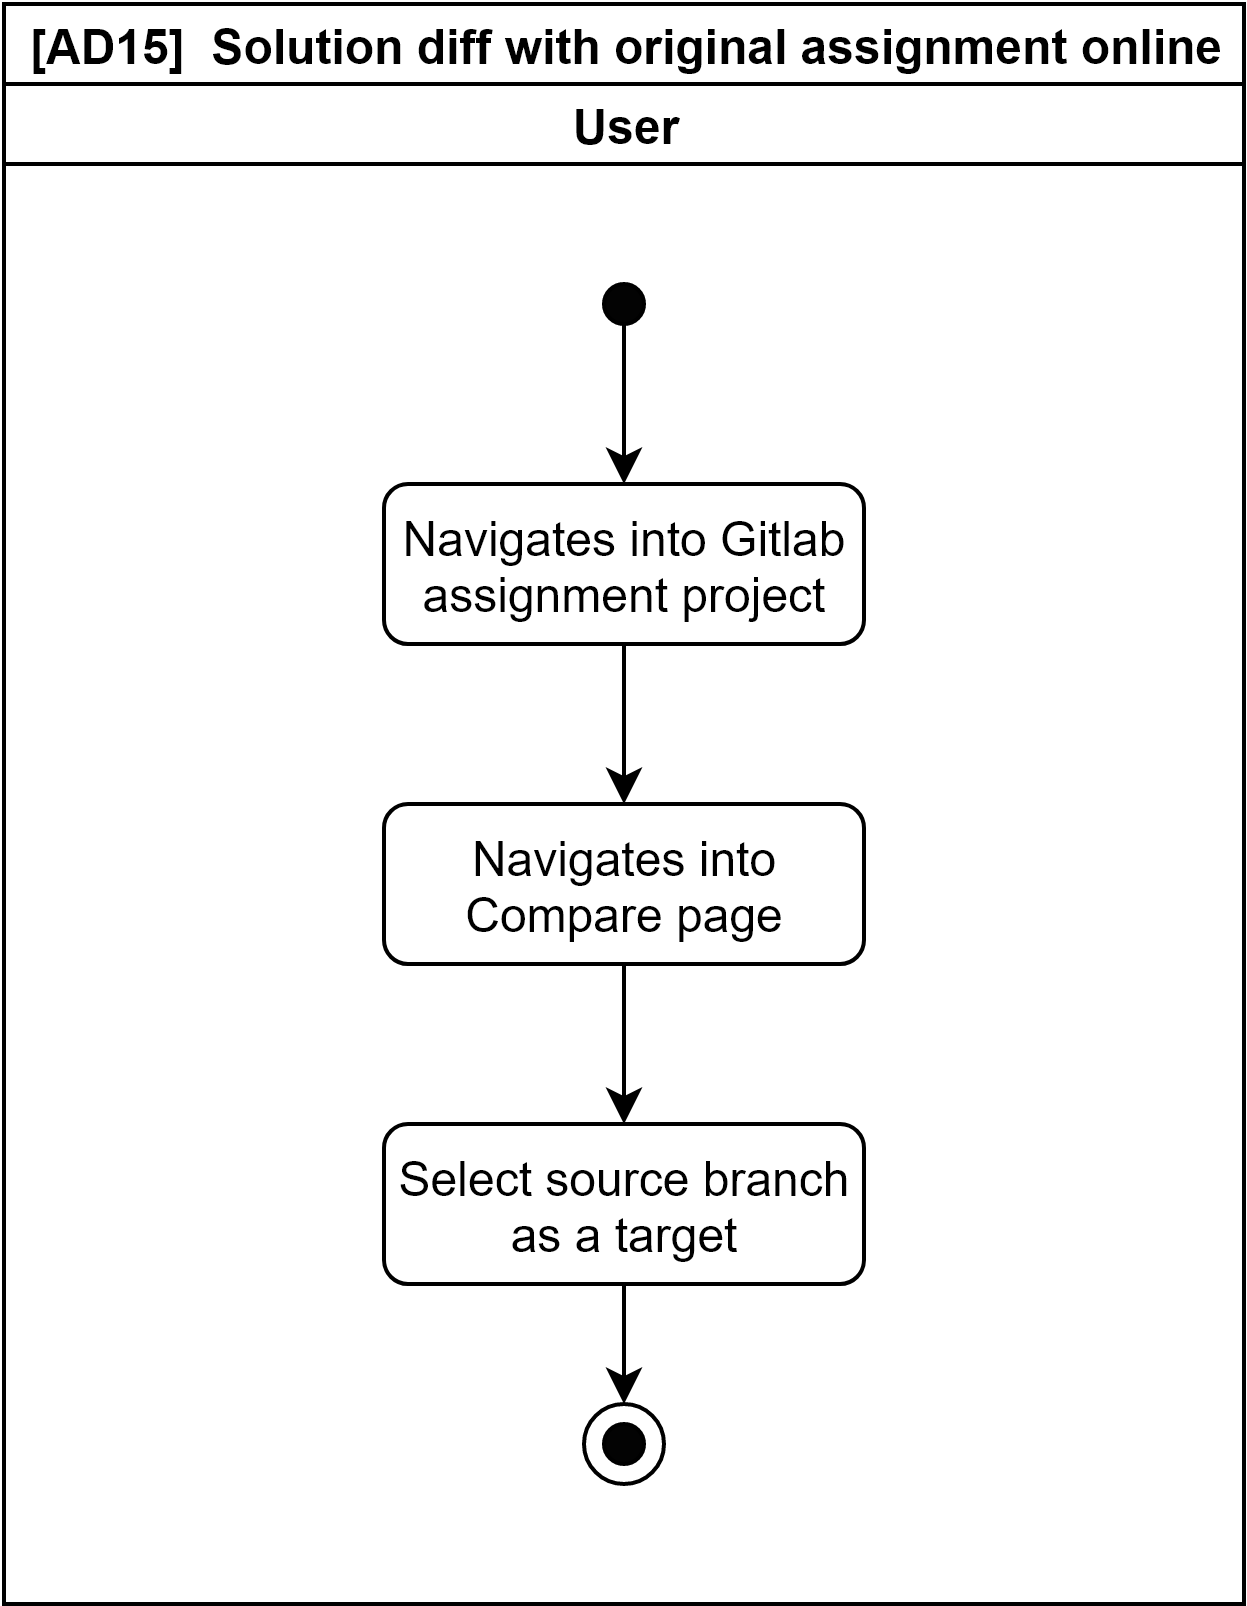
\includegraphics[width=0.6\textwidth,height=\textheight,keepaspectratio]{Figures/ad/ad6.png}
    \caption{~Solution diff with original assignment online activity diagram}
\end{figure}

\subsection{{[}AD16{]} Solution diff with original assignment locally} \label{ssec:ad16}

\begin{figure}[H]
    \centering
    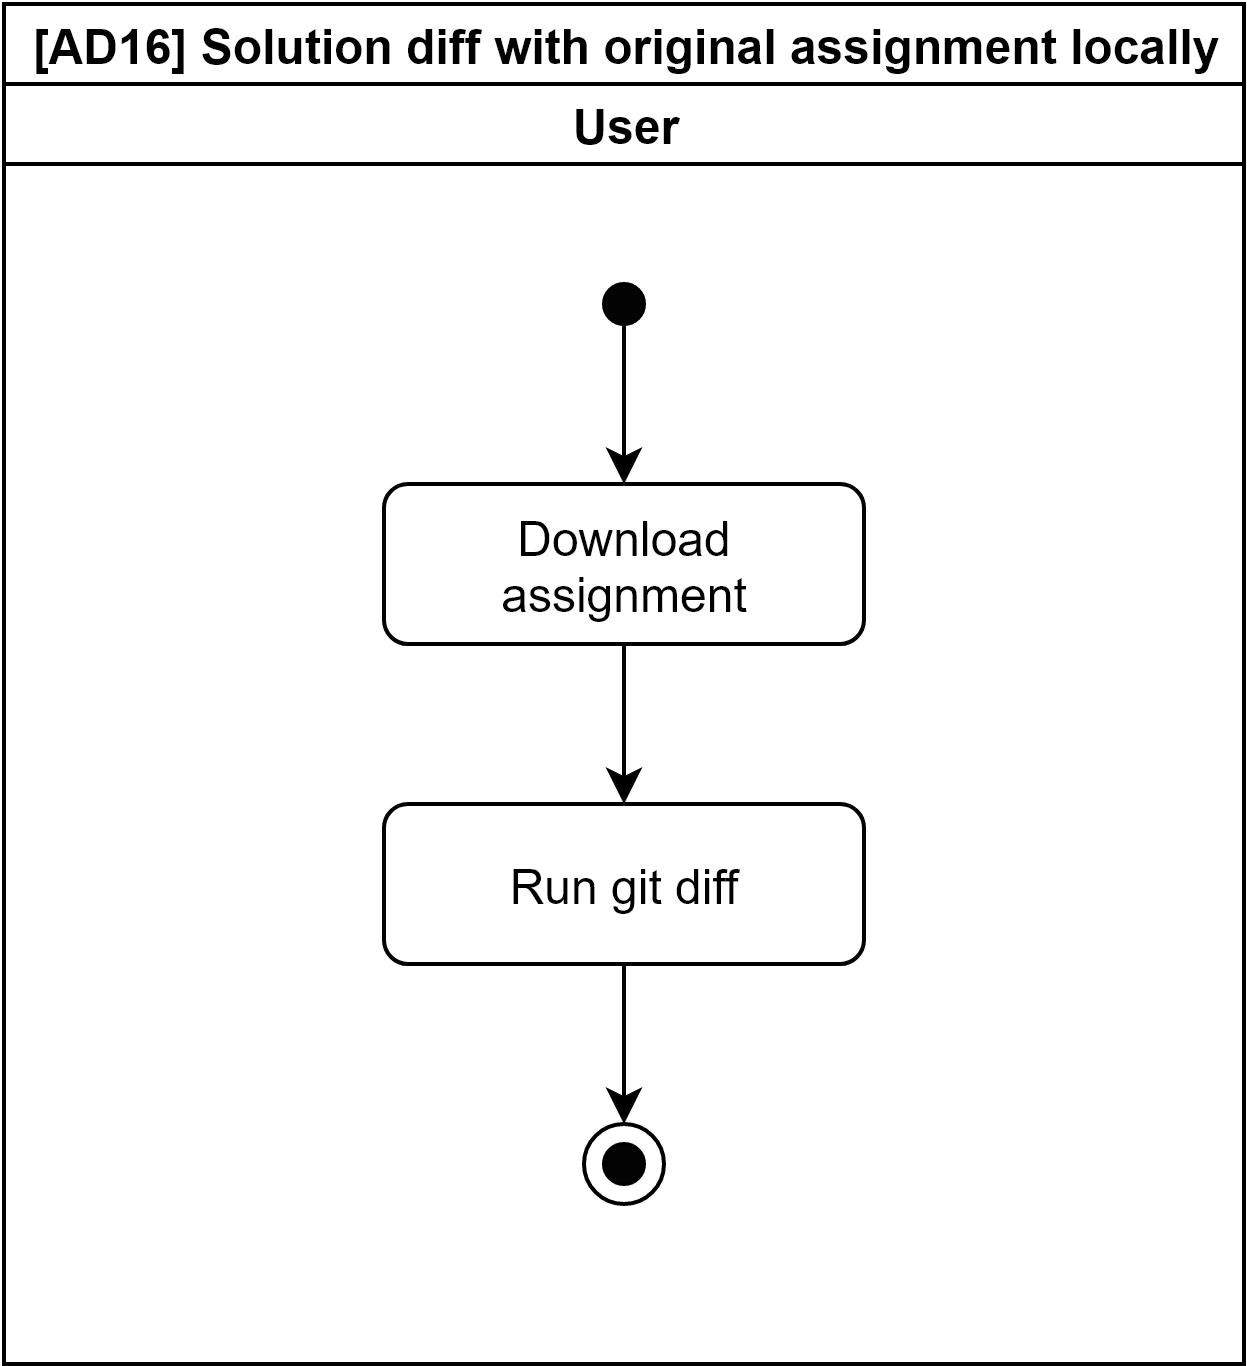
\includegraphics[width=0.6\textwidth,height=\textheight,keepaspectratio]{Figures/ad/ad10.png}
    \caption{Solution diff with original assignment locally activity diagram}
\end{figure}

\subsection{{[}AD17{]} Resolve assignment update with discussion} \label{ssec:ad17}

\begin{figure}[H]
    \centering
    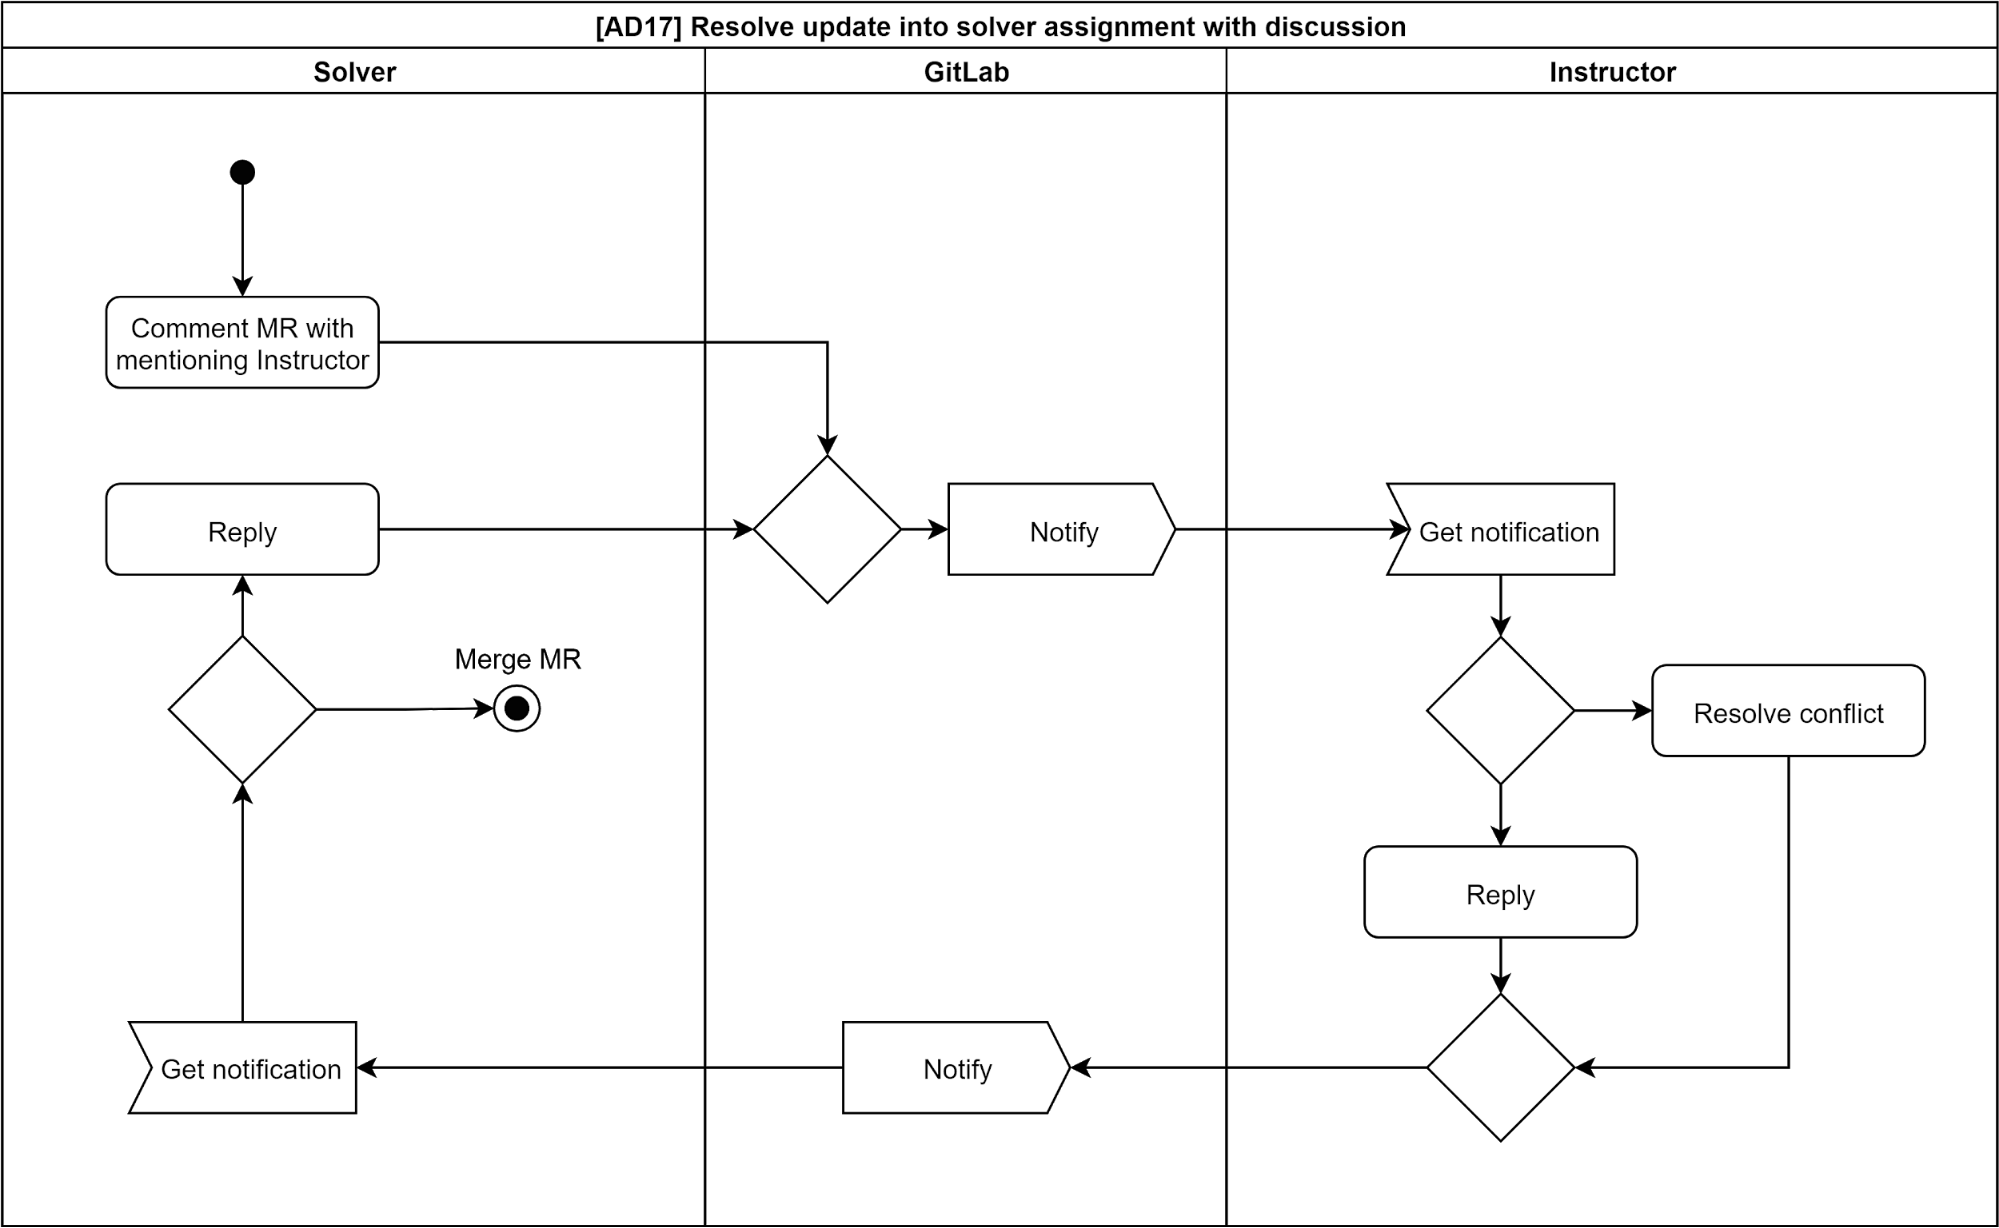
\includegraphics[width=\textwidth,height=\textheight,keepaspectratio]{Figures/ad/ad3.png}
    \caption{Resolve update into solver assignment with discussion activity diagram}
\end{figure}

\section{Use Cases Coverage} \label{sec:ucadc}

The following table shows which use cases are included in individual activity diagrams. It is to ensure that all use cases are covered by activity diagrams.

\begin{table}
    \centering
    \bgroup
    \def\arraystretch{1.5}
    \begin{tabular}{|l|c|c|c|c|c|c|c|c|c|c|c|c|c|}
    \hline
         AD\# & 1\&2 & 3 & 4\&5 & 6\&7 & 8 & 9 & 10 & 11\&17 & 12 & 13 & 14 & 15 & 16 \\ \hline
        IUC1 &  &  &  &  & × &  &  &  &  &  &  &  &  \\ \hline
        IUC4 &  &  &  &  &  & × &  &  &  &  &  &  &  \\ \hline
        IUC5 & × &  &  &  &  &  &  &  &  &  &  &  &  \\ \hline
        IUC6 & × &  &  &  &  &  &  &  &  &  &  &  &  \\ \hline
        IUC7 &  &  & × &  &  &  &  &  &  &  &  &  &  \\ \hline
        IUC8 &  &  &  & × &  &  &  &  &  &  &  &  &  \\ \hline
        IUC10 &  &  &  & × &  &  &  &  &  &  &  &  &  \\ \hline
        IUC11 &  &  &  &  &  &  &  &  &  &  & × &  &  \\ \hline
        GUC1 &  & × &  &  &  &  &  &  &  &  &  &  &  \\ \hline
        GUC3 &  & × &  &  &  &  &  &  &  &  &  &  &  \\ \hline
        GUC4 &  &  &  &  &  &  & × &  &  &  &  &  &  \\ \hline
        GUC5 &  &  &  &  &  &  &  &  &  &  &  & × &  \\ \hline
        GUC6 &  &  &  &  &  &  &  &  &  &  &  &  & × \\ \hline
        SUC1 &  &  &  &  &  &  &  & × &  &  &  &  &  \\ \hline
        SUC2 &  &  &  &  &  &  &  &  & × &  &  &  &  \\ \hline
        SUC3 &  &  &  &  &  &  &  &  &  & × &  &  &  \\ \hline
    \end{tabular}
    \egroup
    \caption{Use Cases and Process Activity Diagrams Coverage}
\end{table}